\documentclass{article}[12pt]
\usepackage{fontspec}   %加這個就可以設定字體
\usepackage{xeCJK}       %讓中英文字體分開設置
\usepackage{indentfirst}
\usepackage{listings}
\usepackage[newfloat]{minted}
\usepackage{float}
\usepackage{graphicx}
\usepackage{caption}
\usepackage{fancyhdr}
\usepackage{hyperref}
\usepackage{amsmath}
\usepackage{multirow}
\usepackage[dvipsnames]{xcolor}
\usepackage{graphicx}
\usepackage{tabularx}
\usepackage{booktabs}
\usepackage{caption}
\usepackage{subcaption}


\usepackage[breakable, listings, skins, minted]{tcolorbox}
\usepackage{etoolbox}
\setminted{fontsize=\footnotesize}
\renewtcblisting{minted}{%
    listing engine=minted,
    minted language=python,
    listing only,
    breakable,
    enhanced,
    minted options = {
        linenos, 
        breaklines=true, 
        breakbefore=., 
        % fontsize=\footnotesize, 
        numbersep=2mm
    },
    overlay={%
        \begin{tcbclipinterior}
            \fill[gray!25] (frame.south west) rectangle ([xshift=4mm]frame.north west);
        \end{tcbclipinterior}
    }   
}

\usepackage[
  top=2cm,
  bottom=2cm,
  left=2cm,
  right=2cm,
  headheight=17pt, % as per the warning by fancyhdr
  includehead,includefoot,
  heightrounded, % to avoid spurious underfull messages
]{geometry} 

\newenvironment{code}{\captionsetup{type=listing}}{}
\SetupFloatingEnvironment{listing}{name=Code}


\title{Introduction to Artificial Intelligence HW 1 Report}
\author{110550088 李杰穎}
\date{\today}

\setCJKmainfont{Noto Serif TC}
\setmonofont[Mapping=tex-text]{Consolas}

\XeTeXlinebreaklocale "zh"             %這兩行一定要加,中文才能自動換行
\XeTeXlinebreakskip = 0pt plus 1pt     %這兩行一定要加,中文才能自動換行

\setlength{\parindent}{0em}
\setlength{\parskip}{2em}
\renewcommand{\baselinestretch}{1.5}
\begin{document}

\maketitle

\section{Code and Explanation}

The following is the code that is required to be finished. Explanation of this code is presented
in the comment of the program.

\begin{code}
\captionof{listing}{Part 1 (\texttt{datasets.py})}
\begin{minted}
import os
import cv2
import numpy as np
def loadImages(dataPath):
    """
    Load all Images in the folder and transfer a list of tuples. 
    The first element is the numpy array of shape (m, n) representing the image.
    (remember to resize and convert the parking space images to 36 x 16 grayscale images.) 
    The second element is its classification (1 or 0)
        Parameters:
        dataPath: The folder path.
        Returns:
        dataset: The list of tuples.
    """
    # Begin your code (Part 1)
    dataset = [] # Declare an empty list to save the grayscale images

    # Process images in "car" directory
    for item in os.listdir(os.path.join(dataPath, "car")): # Use os.path.join to generate paths
        img = cv2.imread(os.path.join(dataPath, "car", item)) # Read image from files
        img = cv2.resize(img, (36, 16)) # Resize the image from (360, 160) to (36, 16)
        img = cv2.cvtColor(img, cv2.COLOR_BGR2GRAY) # Convert image to grayscale image
        data = (img, 1) # Create a tuple to store image and label and 
        # because all images in "car" folder is the occupied parking space, the label is set to 1
        dataset.append(data) # Append the tuple to the dataset list
    
    for item in os.listdir(os.path.join(dataPath, "non-car")): # Do the same thing as above but this time is for "non-car" folder
        img = cv2.imread(os.path.join(dataPath, "non-car", item))
        img = cv2.resize(img, (36, 16))
        img = cv2.cvtColor(img, cv2.COLOR_BGR2GRAY)
        data = (img, 0) # Not occupied parking space, label is set to 0
        dataset.append(data)
    # End your code (Part 1)
    
    return dataset

\end{minted}
\end{code}

\begin{code}
\captionof{listing}{Part 2 (\texttt{adaboost.py/selectBest})}
\begin{minted}
def selectBest(self, featureVals, iis, labels, features, weights):
"""
Finds the appropriate weak classifier for each feature.
Selects the best weak classifier for the given weights.
    Parameters:
    featureVals: A numpy array of shape (len(features), len(dataset)).
        Each row represents the values of a single feature for each training sample.
    iis: A list of numpy array with shape (m, n) representing the integral images.
    labels: A list of integer.
        The ith element is the classification of the ith training sample.
    features: A numpy array of HaarFeature class.
    weights: A numpy array with shape(len(dataset)).
        The ith element is the weight assigned to the ith training sample.
    Returns:
    bestClf: The best WeakClassifier Class
    bestError: The error of the best classifer
"""
# Begin your code (Part 2)
# Init. WeakClassifier by the feature in features list
# And append them all into the clfs list
clfs = [WeakClassifier(feature=feature) for feature in features]

# Declare bestClf and bestError to store the currently best classifier and its error
bestClf = None
bestError = sum(weights) # The max error is the sum of weights

for clf in clfs: # Iterate all classifer in clfs
    error = 0    # Declare a variable to track the error of the current clf
    for i in range(len(iis)): # Iterate all image sample
        if clf.classify(iis[i]) != labels[i]: # When the prediction of the model is different with the lable
            error += weights[i] # Add weights to error
    if error < bestError: # If the error is smaller than the best error, then classifier is the currently best classifer
        bestError = error # Change bestError to current error
        bestClf = clf     # Save this classifier as bestClf

# End your code (Part 2)
return bestClf, bestError
\end{minted}
\end{code}

\begin{code}
\captionof{listing}{Part 3 (\texttt{main.py})}
\begin{minted}
print('Start training your classifier')
for t in range(1, 11): # Train with different T (1 ~ 10)
    print(f"Training with T={t}") 
    clf = adaboost.Adaboost(T=t) # Init. clf using the given T
    clf.train(trainData) # Train of train data
    clf.save(f'clf_300_{t}') # Save the model file as clf_300_<t>
    clf = adaboost.Adaboost.load(f'clf_300_{t}') # Load the model after saving

    # Evaluate the model using already written utils.evaluate function
    print('\nEvaluate your classifier with training dataset')
    utils.evaluate(clf, trainData) # Use train data to evaluate model

    print('\nEvaluate your classifier with test dataset')
    utils.evaluate(clf, testData) # Use test data to evaluate model

    # Part 4: Implement detect function in detection.py and test the following code.
    print('\nUse your classifier with video.gif to get the predictions (one .txt and one .png)')
    detection.detect('data/detect/detectData.txt', clf, t) # Save the detection results to detectData.txt
\end{minted}
\end{code}

\begin{code}
\captionof{listing}{Part 4 (\texttt{detection.py/detect})}
\begin{minted}
def detect(dataPath, clf, t=10):
    """
    Please read detectData.txt to understand the format. 
    Use cv2.VideoCapture() to load the video.gif.
    Use crop() to crop each frame (frame size = 1280 x 800) of video to get parking space images. (image size = 360 x 160) 
    Convert each parking space image into 36 x 16 and grayscale.
    Use clf.classify() function to detect car, If the result is True, draw the green box on the image like the example provided on the spec. 
    Then, you have to show the first frame with the bounding boxes in your report.
    Save the predictions as .txt file (Adaboost_pred.txt), the format is the same as GroundTruth.txt. 
    (in order to draw the plot in Yolov5_sample_code.ipynb)
    
      Parameters:
        dataPath: the path of detectData.txt
      Returns:
        No returns.
    """
    # Begin your code (Part 4)
    cords = [] # Declare a list that stores the cordinate of each parking slots
    with open(dataPath) as file:
        num_of_parking = int(file.readline()) # Read the number total parking slots from the first line of files
        for _ in range(num_of_parking): # Iterate all lines
            tmp = file.readline() # Read a line in file
            tmp = tmp.split(" ") # Split the line using " "
            res = tuple(map(int, tmp)) # Convert the string type to int type using the built-in map function
            cords.append(res) # Append the cordinates to "cords" list
    
    cap = cv2.VideoCapture(os.path.join(dataPath, "..", "video.gif")) # Use cv2.VideoCapture to read video.gif
    frame = 0 # Counter to track current frame number
    output_gif = [] # Declare a list to store each processed frame of output.gif
    first_frame = True # A flag that will help us store the processed first frame images
    while True:
        detect_label = [] # Declare a list to store the detect results of each parking slots
        frame += 1 # Make frame number add 1
        _, img = cap.read() # Read a frame of video.gif
        if img is None: # If all frame are read, then img is None
            break # If None, then break
        for cord in cords: # Iterate all cords
            pic = crop(*cord, img) # Use * to unpack cord e.g. (x1, y1, ..., x4, y4) -> x1, y1, ..., x4, y4
            pic = cv2.resize(pic, (36, 16)) # Resize image to (36, 16)
            pic = cv2.cvtColor(pic, cv2.COLOR_RGB2GRAY) # Convert image to grayscale images
            detect_label.append(clf.classify(pic)) # Use clf.classify to detect whether the parking slot is occupied or not and append the result to "detect_label" list
        for i, label in enumerate(detect_label): # Iterate all detect_label
            if label: # If the model detects that this parking slot is occupied
                pos = [[cords[i][idx], cords[i][idx+1]] for idx in range(0, 8, 2)] # Add the four points of the rectangle to "pos" list
                pos[2], pos[3] = pos[3], pos[2] # swap pos[2] and pos[3]
                pos = np.array(pos, np.int32) # Convert python built-in list to numpy array
                cv2.polylines(img, [pos], color=(0, 255, 0), isClosed=True) # Use cv2.polylines to draw rectangle
    
        output_gif.append(cv2.cvtColor(img, cv2.COLOR_BGR2RGB)) # Append the result image of each frame to output_gif list (Also convert the color)
        if first_frame: # If this frame is the first frame in video.gif
            first_frame = False # After getting into this block, set first_frame to False
            cv2.imwrite(f"Adaboost_first_frame_{t}.png", img) # Save the results of first frame
        with open(f"Adaboost_pred_{t}.txt", "a") as txt: # Open the Adaboost_pred_<t>.txt and use append mode to add new line to file
            res = "" # Declare an empty string
            for i, label in enumerate(detect_label): # Iterate all labels
                if label:
                    res += "1" # If the parking slot is occupied, then write 1 to file
                else:
                    res += "0" # Else write 1
                if i != len(detect_label) - 1:
                    res += " " # If not the last label in a frame, then write a space to seperate each label
                else:
                    res += "\n" # Else write newline character
            txt.write(res) # Write the res string to file
    imageio.mimsave(f'results_{t}.gif', output_gif, fps=2) # Use imageio.imsave to save result gif and set fps to 2
    # End your code (Part 4)

\end{minted}
\end{code}

\begin{code}
\captionof{listing}{Part 5 (\texttt{yolov5\_sample\_code.ipynb})}
\begin{minted}
dataPath = os.path.join("HW1_material", "detect", "detectData.txt") # Path to "detectData.txt"
cords = [] # Declare a list that stores the cordinate of each parking slots
with open(dataPath) as file: # Open "detectData.txt"
    num_of_parking = int(file.readline()) # Read the number total parking slots from the first line of files
    for _ in range(num_of_parking): # Iterate all lines
        tmp = file.readline() # Read a line in file
        tmp = tmp.split(" ") # Split the line using " "
        res = tuple(map(int, tmp)) # Convert the string type to int type using the built-in map function
        cords.append(res) # Append the cordinates to "cords" list

cap = cv2.VideoCapture(os.path.join("HW1_material", "detect", "video.gif")) # Use cv2.VideoCapture to read video.gif
frame = 0 # Counter to track current frame number
output_gif = [] # Declare a list to store each processed frame of output.gif
first_frame = True # A flag that will help us store the processed first frame images
while True:
    detect_label = [] # Declare a list to store the detect results of each parking slots
    frame += 1 # Make frame number add 1
    _, img = cap.read() # Read a frame of video.gif
    if img is None: # If all frame are read, then img is None
        break # If None, then break
    for cord in cords: # Iterate all cords
        pic = crop(*cord, img) # Use * to unpack cord e.g. (x1, y1, ..., x4, y4) -> x1, y1, ..., x4, y4
        pic = cv2.resize(pic, (36, 16)) # Resize image to (36, 16)
        detect_label.append(yolov5_func.classify(pic, weight_path, confidence_threshold, (36, 16))) # Use yolov5_func.classify to detect whether the parking slot is occupied or not, and append the result to "detect_label" list
    for i, label in enumerate(detect_label): # Iterate all detect_label
        if label: # If the model detects that this parking slot is occupied
            pos = [[cords[i][idx], cords[i][idx+1]] for idx in range(0, 8, 2)] # Add the four points of the rectangle to "pos" list
            pos[2], pos[3] = pos[3], pos[2] # swap pos[2] and pos[3]
            pos = np.array(pos, np.int32) # Convert python built-in list to numpy array
            cv2.polylines(img, [pos], color=(0, 255, 0), isClosed=True) # Use cv2.polylines to draw rectangle

    output_gif.append(cv2.cvtColor(img, cv2.COLOR_BGR2RGB)) # Append the result image of each frame to output_gif list (Also convert the color)
    if first_frame: # If this frame is the first frame in video.gif
        cv2.imwrite(img_save_path, img) # After getting into this block, set first_frame to False
        first_frame = False # Save the results of first frame
    with open(txt_save_path, "a") as txt: # Open txt file and use append mode to add new line to file 
        res = "" # Declare an empty string
        for i, label in enumerate(detect_label): # Iterate all labels
            if label:
                res += "1" # If the parking slot is occupied, then write 1 to file
            else:
                res += "0" # Else write 1
            if i != len(detect_label) - 1:
                res += " " # If not the last label in a frame, then write a space to seperate each label
            else:
                res += "\n" # Else write newline character
        txt.write(res) # Write the res string to file
imageio.mimsave(gif_save_path, output_gif, fps=2) # Use imageio.imsave to save result gif and set fps to 2
\end{minted}
\end{code}

\section{Experiments}
\subsection{Hyperparameters Adjustment}
\subsubsection{Adaboost}
In Adaboost algorithm, I only change the hyperparameter \texttt{T}, 
which indicates the number of classifers that will be used in the training process.

I have trained 10 models, from $T=1$ to $T=10$. The performance of these 10 models will be
shown in Section \ref{subsec:ada_comp}.

\subsubsection{YOLOv5}
In YOLOv5, the only hyperparameter I can change is the confidence threshold, which is a
probability threshold. If the YOLOv5's output is greater than the threshold, then it considers
that the parking slot is occupied.

I have tested three kinds of threshold, which are 0.3, 0.4 and 0.5. And the performance of these
three value will be presented in Section \ref{subsec:yolo_comp}.

\section{Results} \label{sec:res}
\subsection{Measurements}
\subsubsection{Accuracy}
In binary classification problem, we often define four kinds of accuracy, 
which are True Positive, True Negative, False Positive, and False Negative 
to show the performance of classifiers. Their definitions are written below:
\begin{itemize}
    \item True Positive (TP): The real label is \textbf{true}, 
    and our model predicts that it's \textbf{true}.
    \item True Negative (TN): The real label is \textbf{false}, 
    and our model predicts that it's \textbf{false}.
    \item False Positive (FP): The real label is \textbf{true}, 
    but our model predicts that it's \textbf{false}.
    \item False Negative (FN): The real label is \textbf{false}, 
    but our model predicts that it's \textbf{true}.
\end{itemize}
\subsubsection{F-Score}
F-score is used to measure a test's accuracy. 
To define F-score, we first need to define two variables, 
``precision'' and ``recall''.

\begin{equation}
    \text {precision}=\frac{\text{TP}}{\text{TP}+\text{FP}}
\end{equation}

\begin{equation}
    \text {recall}=\frac{\text{TP}}{\text{TP}+\text{FN}}
\end{equation}

And the definition of F-score is:

\begin{equation}
    \text {F-score}=\frac{\left(1+\beta^{2}\right) \text { precision } \times \text { recall }}{\beta^{2} \text { precision }+\text { recall }}
\end{equation}

In reality, we often use ``F1-score'', which means $\beta=1$. Therefore, the ``F1-score'' can be written as:
\begin{equation}
    \text {F1-score}=2 \times \frac{\text { precision } \times \text { recall }}{\text { precision }+\text { recall }}
\end{equation}

The range of F1-score is $[0, 1]$. If F1-score is higher (closer to 1), 
then the performance of classifier is better.

\subsection{Adaboost Comparision} \label{subsec:ada_comp}

\begin{table}[H]
    \centering    
    \caption{Performance of different Adaboost model from $T=1$ to $T=10$ on training datasets}
    \begin{tabular}{@{}ccccccc@{}}
        \toprule
        $T$  & FP Rate (\%)  & FN Rate (\%)   & Accuracy (\%)  & Precision (\%)   & Recall (\%)      & F1-score         \\ \midrule
        1  & 8.33          & 29.00          & 81.33          & 91.67        & 75.97        & 83.08        \\
        2  & 8.33          & 29.00          & 81.33          & 91.67        & 75.97        & 83.08        \\
        3  & \textbf{4.33} & 23.33          & 81.50          & \textbf{95.67}        & 80.39        & 87.37        \\
        4  & 9.00          & 17.00          & 87.00          & 91.00        & 84.26        & 87.50        \\
        5  & 7.00          & 13.33          & 89.83          & 92.33        & 88.50        & 90.38        \\
        6  & 8.00          & 12.00 & 90.00          & 92.00        & 88.46        & 90.20        \\
        7  & 7.00          & 13.33          & 89.83          & 93.00 & 87.46        & 90.15        \\
        8  & 7.00          & 12.00 & 90.50          & 93.00        & 88.57        & 90.73        \\
        9  & 8.00          & \textbf{10.67}          & \textbf{90.67} & 92.00        & \textbf{89.61} & \textbf{90.79} \\
        10 & 7.33          & 12.67          & 90.00          & 92.67        & 87.97        & 90.26        \\ \bottomrule
        \end{tabular}
        \label{tab:ada_train}
\end{table}

\begin{table}[H]
    \centering
    \caption{Performance of different Adaboost model from $T=1$ to $T=10$ on testing datasets}
    \begin{tabular}{@{}ccccccc@{}}
        \toprule
        $T$  & FP Rate (\%)  & FN Rate (\%)   & Accuracy (\%)  & Precision (\%)   & Recall (\%)      & F1-score  \\ \midrule
        1  & 8.00          & 30.33          & 80.83          & 92.00         & 75.20         & 82.76         \\
        2  & 8.00          & 30.33          & 80.83          & 92.00         & 75.20         & 82.76         \\
        3  & 6.33          & 30.67          & 81.50          & \textbf{93.67} & 75.34         & 83.51         \\
        4  & 9.00          & 22.67          & 84.17          & 91.00         & 80.06         & 85.18         \\
        5  & 8.67          & 21.00          & 85.17          & 91.33         & 81.31         & 86.03         \\
        6  & \textbf{8.33} & \textbf{19.33} & \textbf{86.17} & 91.67         & \textbf{82.58} & \textbf{86.89} \\
        7  & 7.67          & 23.67          & 84.33          & 92.33         & 79.60         & 85.49         \\
        8  & 7.67          & 21.67          & 85.33          & 92.33         & 80.99         & 86.29         \\
        9  & 10.00         & 20.00          & 85.00          & 90.00         & 81.82         & 85.71         \\
        10 & 8.33          & 20.67          & 85.50          & 91.67         & 81.60         & 86.34         \\ \bottomrule
    \end{tabular}
    \label{tab:ada_test}    
\end{table}

From Table \ref{tab:ada_test}, we can observe that when $T=6$, the F1-score is the highest.

This means the best value for hyperparameter $T$ is 6. Therefore, in the comparision of Adaboost
and YOLOv5, I will set $T=6$ to compare with YOLOv5.
\subsection{YOLOv5 Comparison} \label{subsec:yolo_comp}

% Please add the following required packages to your document preamble:
% \usepackage{booktabs}
\begin{table}[H]
    \centering
    \caption{Performance of different confidence threshold on training datasets}
    \begin{tabular}{@{}ccccccc@{}}
    \toprule
    Threshhold & FP Rate (\%)  & FN Rate (\%)  & Accuracy (\%)  & Precision (\%) & Recall (\%)     & F1-score       \\ \midrule
    0.1 & 32.00 & 0.00 & 84.00 & 68.00 & 100.00 & 80.95 \\
    0.2 & 24.67 & 0.00 & 87.67 & 75.33 & 100.00 & 85.93 \\
    0.3        & 19.67         & \textbf{0.00} & 90.17          & 80.33          & \textbf{100.00} & 89.09          \\
    0.4        & 12.00         & 0.33          & 93.83          & 88.00          & 99.62           & 93.45          \\
    0.5        & 2.67          & 7.00          & \textbf{95.17} & 97.33          & 93.29           & \textbf{95.27} \\
    0.6        & \textbf{0.67} & 67.33         & 66.00          & \textbf{99.33} & 59.60           & 74.50          \\ \bottomrule
    \end{tabular}
    \label{tab: yolo_train}
\end{table}

\begin{table}[H]
    \centering
    \caption{Performance of different confidence threshold on testing datasets}
    \begin{tabular}{@{}ccccccc@{}}
    \toprule
    Threshhold & FP Rate (\%)  & FN Rate (\%)  & Accuracy (\%)  & Precision (\%)  & Recall (\%)     & F1-score       \\ \midrule
    0.1 & 30.00 & 0.00 & 85.00 & 70.00 & 100.00 & 82.35 \\
    0.2 & 19.67 & 0.00 & 90.17 & 80.33 & 100.00 & 89.09 \\
    0.3        & 13.00         & \textbf{0.00} & 93.50          & 87.00           & \textbf{100.00} & 93.05          \\
    0.4        & 5.00          & 0.00          & 97.50          & 95.00           & 100.00          & 97.44          \\
    0.5        & 1.67          & 1.00          & \textbf{98.67} & 98.33           & 98.99           & \textbf{98.66} \\
    0.6        & \textbf{0.00} & 59.00         & 70.50          & \textbf{100.00} & 62.89           & 77.22          \\ \bottomrule
    \end{tabular}
    \label{tab: yolo_test}
\end{table}

From Table \ref{tab: yolo_train} and Table \ref{tab: yolo_test}, 
we can observe that when the confidence threshold equals to 0.5, the F1-score on both
training and testing is the highest.

This means the best value for the hyperparameter ``confidence threshold'' is 0.5.
Therefore, in the comparison of Adaboost and YOLOv5, I will set the confidence threshold to 0.5
when comparing with Adaboost.

\subsection{Comparision between Adaboost and YOLOv5}

\begin{table}[H]
    \centering
    \caption{Performance of Adaboost and YOLOv5 on testing datasets}
    \begin{tabular}{@{}ccccccc@{}}
    \toprule
    Model    & FP Rate (\%)  & FN Rate (\%)  & Accuracy (\%)  & Precision (\%) & Recall (\%)    & F1-score       \\ \midrule
    Adaboost & 8.33          & 19.33         & 86.17          & 91.67          & 82.58          & 86.89          \\
    YOLOv5   & \textbf{1.67} & \textbf{1.00} & \textbf{98.67} & \textbf{98.33} & \textbf{98.99} & \textbf{98.66} \\ \bottomrule
    \end{tabular}
    \label{tab:com_ada_yolo}
\end{table}

From Table \ref{tab:com_ada_yolo}, we can observe that YOLOv5 outperforms the traditional
Adaboost method.

\subsection{The detection result of a real parking lot}

The figures and plots below are the detection result of the parking lot. I use different
hyperparameters and models to detect the occupied parking slots. I will also compare the 
performance of each model.

\subsubsection{Plots}

\begin{figure}[H]
    \centering
    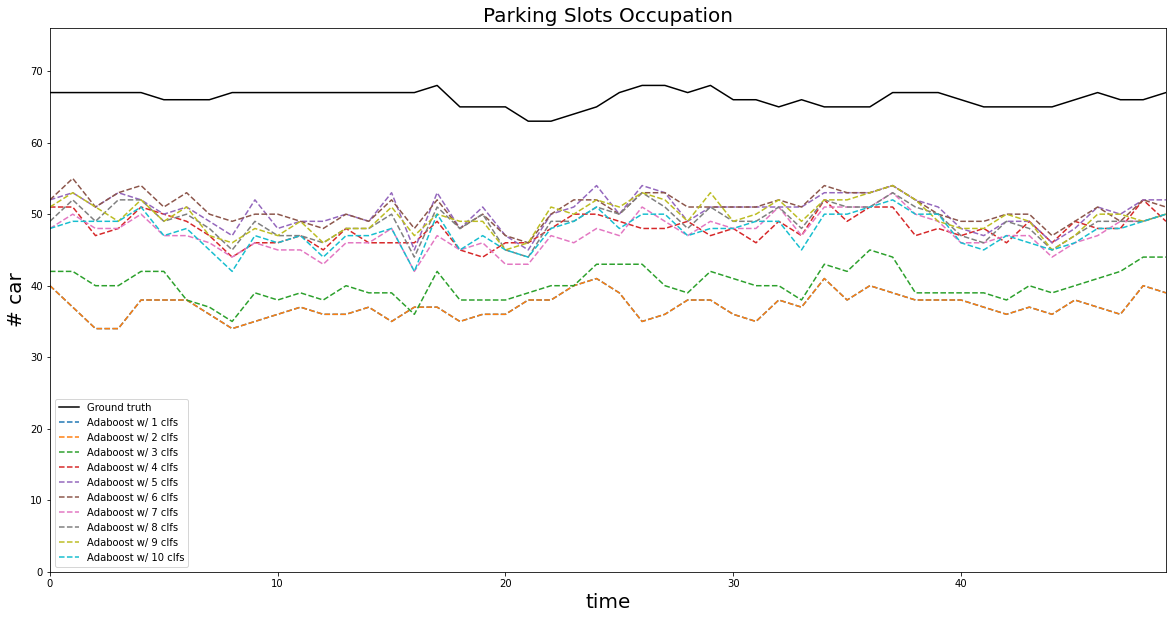
\includegraphics[width=0.75\textwidth]{figure/Parking_Slots_Occupation_Adaboost.png}
    \caption{The number of occupied parking slots detected by Adaboost ($T=1$ to $T=10$) 
    and the ground truth}
\end{figure}

\begin{figure}[H]
    \centering
    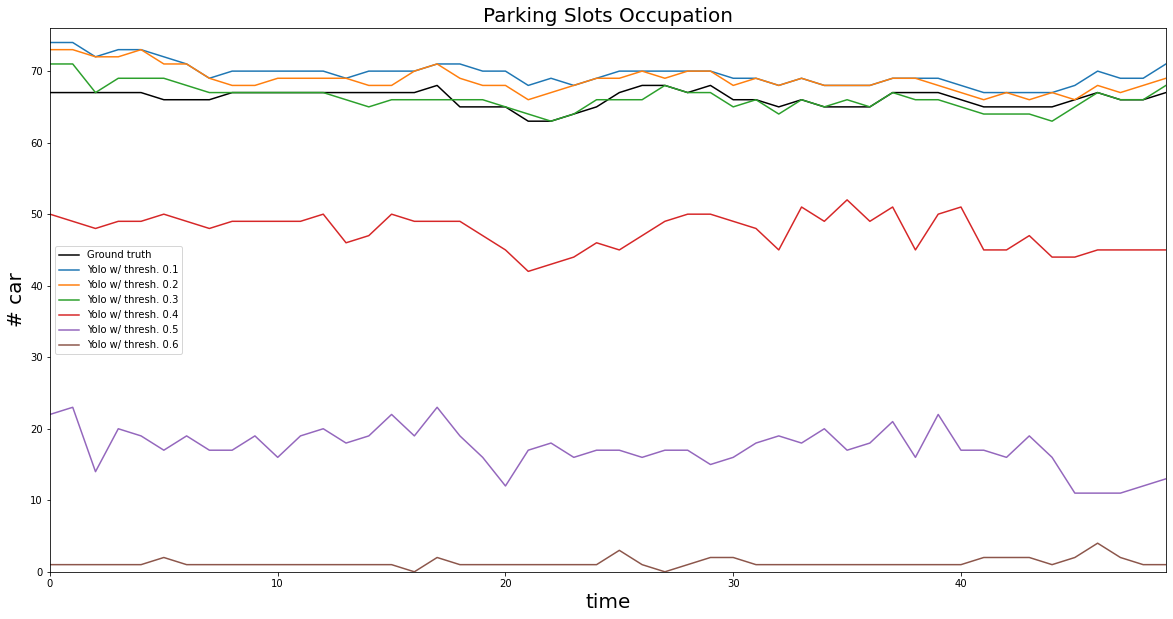
\includegraphics[width=0.75\textwidth]{figure/Parking_Slots_Occupation_yolo.png}
    \caption{The number of occupied parking slots detected by YOLOv5 ($\text{threshold}=0.1$ 
    to $\text{threshold}=0.6$) and the ground truth}
\end{figure}

\begin{figure}[H]
    \centering
    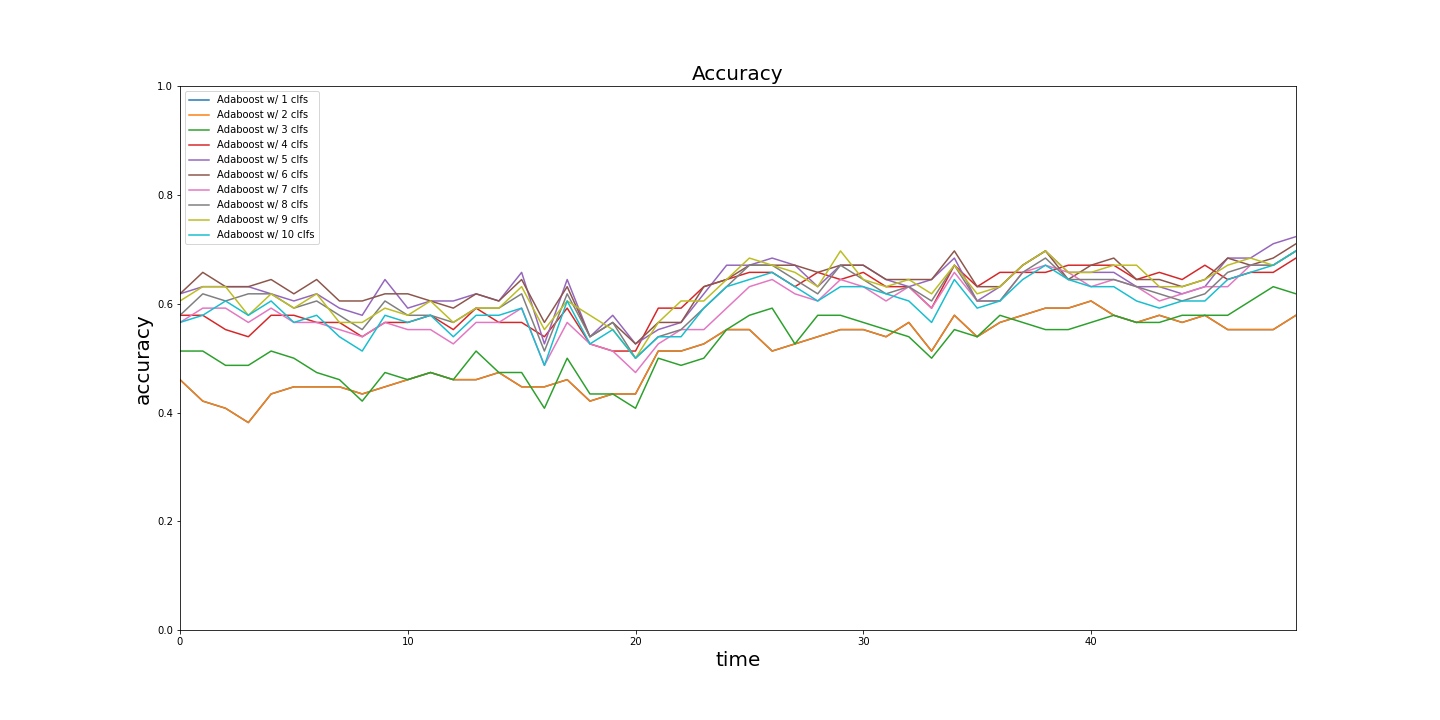
\includegraphics[width=0.75\textwidth]{figure/Accuracy_Adaboost.png}
    \caption{Accuracy of Adaboost ($T=1$ to $T=10$) over time}
    \label{fig:acc_ada}
\end{figure}

\begin{figure}[H]
    \centering
    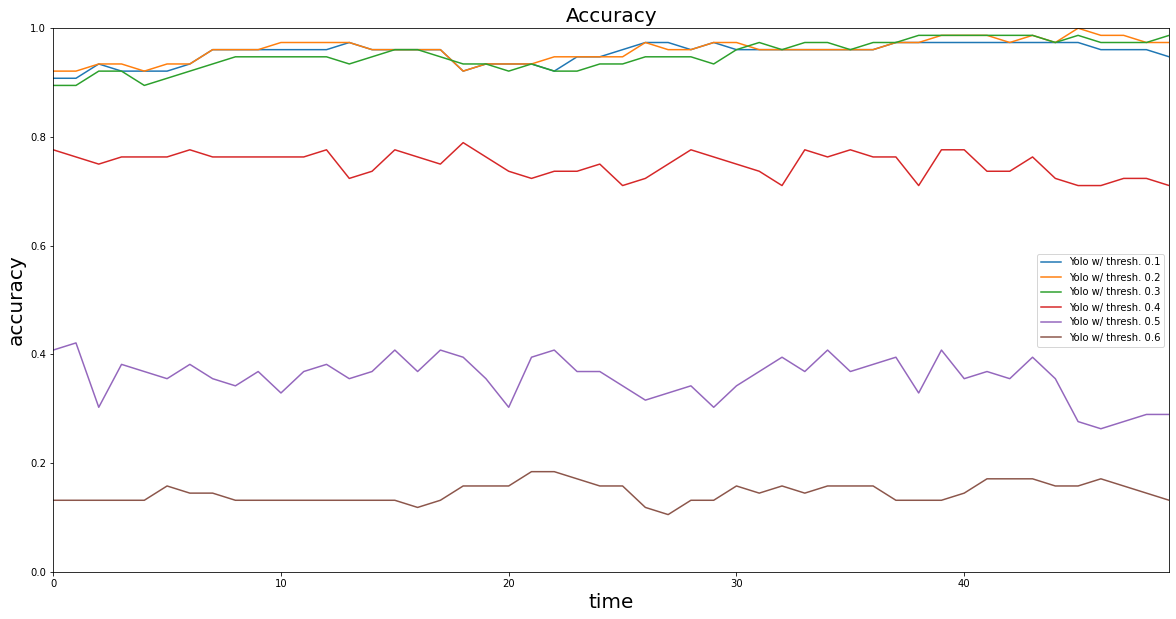
\includegraphics[width=0.75\textwidth]{figure/Accuracy_yolo.png}
    \caption{Accuracy of YOLOv5 ($\text{threshold}=0.1$ 
    to $\text{threshold}=0.6$) over time}
    \label{fig:acc_yolo}
\end{figure}

\begin{figure}[H]
    \centering
    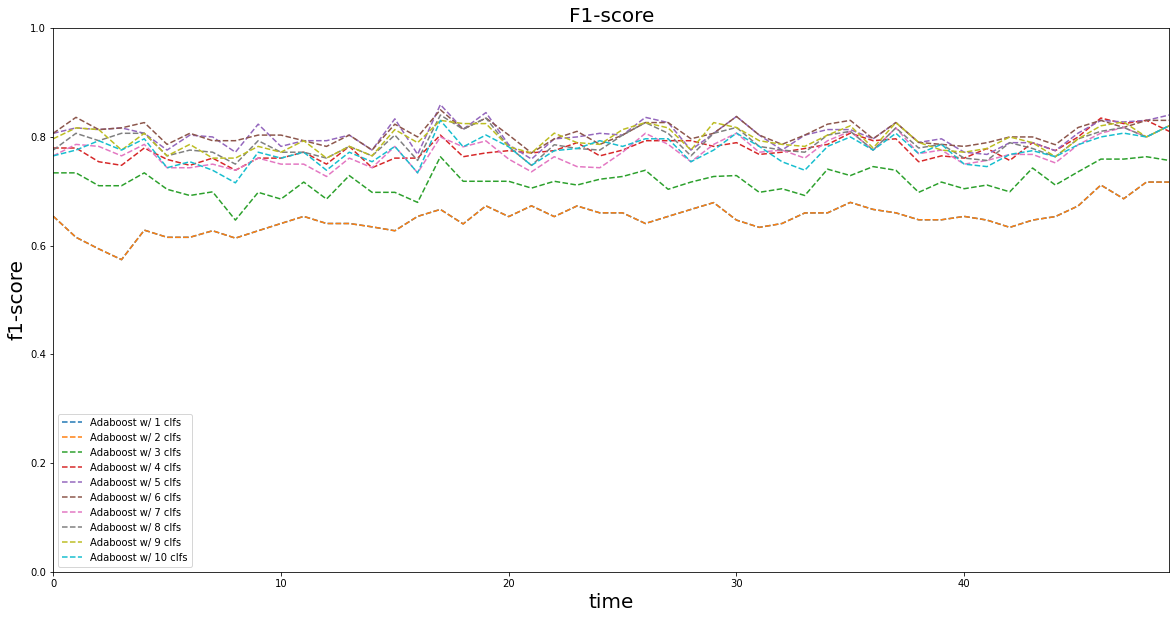
\includegraphics[width=0.75\textwidth]{figure/F1-score_Adaboost.png}
    \caption{F1-score of Adaboost ($T=1$ to $T=10$) over time}
    \label{fig:f1_ada}
\end{figure}

\begin{figure}[H]
    \centering
    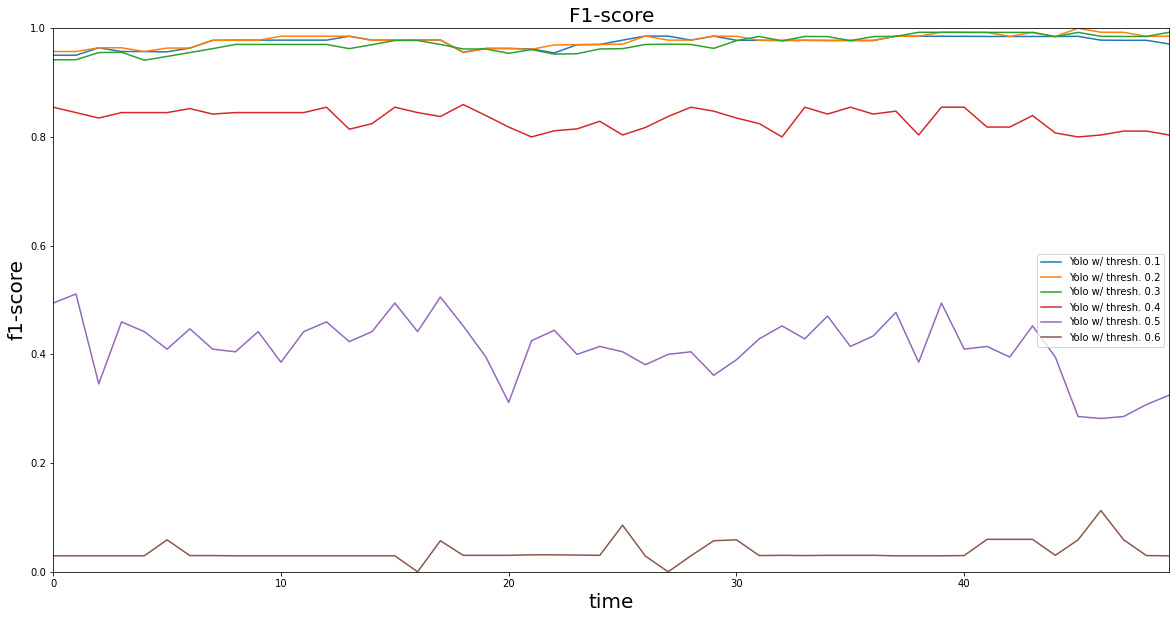
\includegraphics[width=0.75\textwidth]{figure/F1-score_yolo.png}
    \caption{F1-score of YOLOv5 ($\text{threshold}=0.1$ 
    to $\text{threshold}=0.6$) over time}
    \label{fig:f1_yolo}
\end{figure}

\begin{figure}[H]
    \centering
    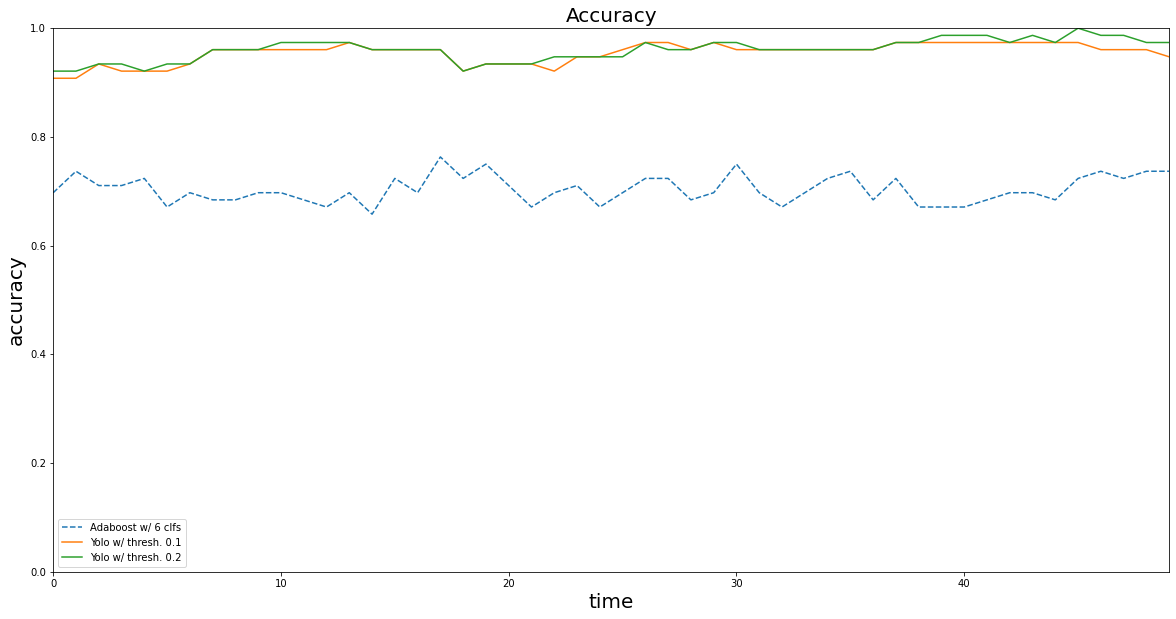
\includegraphics[width=0.75\textwidth]{figure/Accuracy_all.png}
    \caption{Accuracy of Adaboost ($T=6$) and YOLOv5 ($\text{threshold}=0.1, 0.2$) over time}
    \label{fig:acc_all}
\end{figure}

\begin{figure}[H]
    \centering
    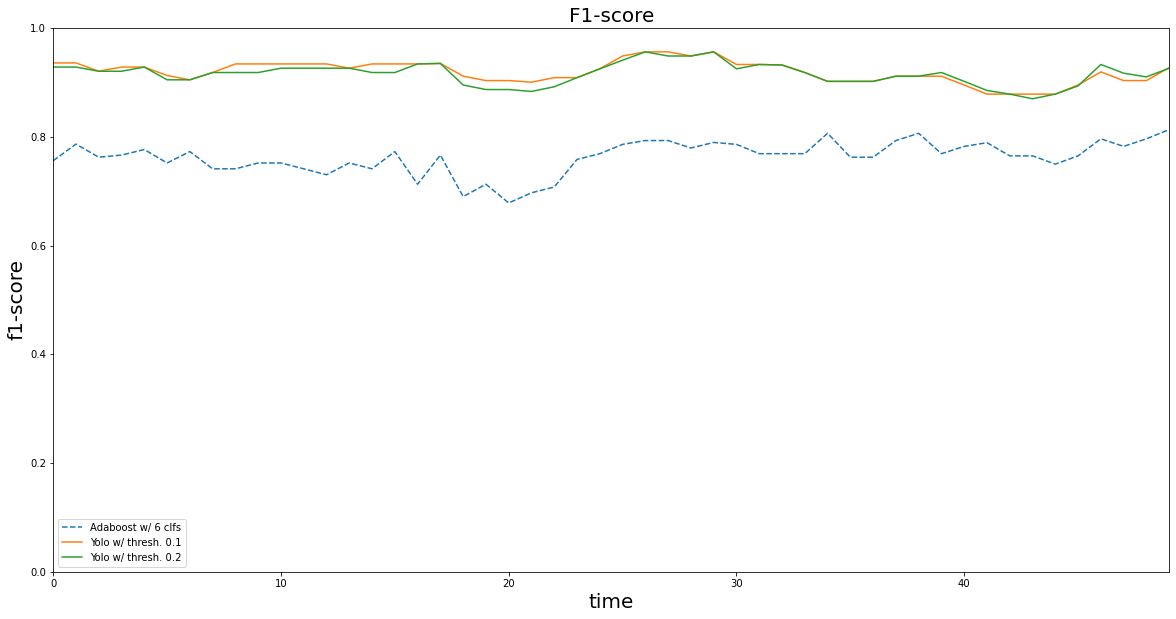
\includegraphics[width=0.75\textwidth]{figure/F1-score_all.png}
    \caption{F1-score of Adaboost ($T=6$) and YOLOv5 ($\text{threshold}=0.1, 0.2$) over time}
    \label{fig:f1_all}
\end{figure}

\subsubsection{The first frame of video.gif}

\begin{figure}[H]
    \centering
    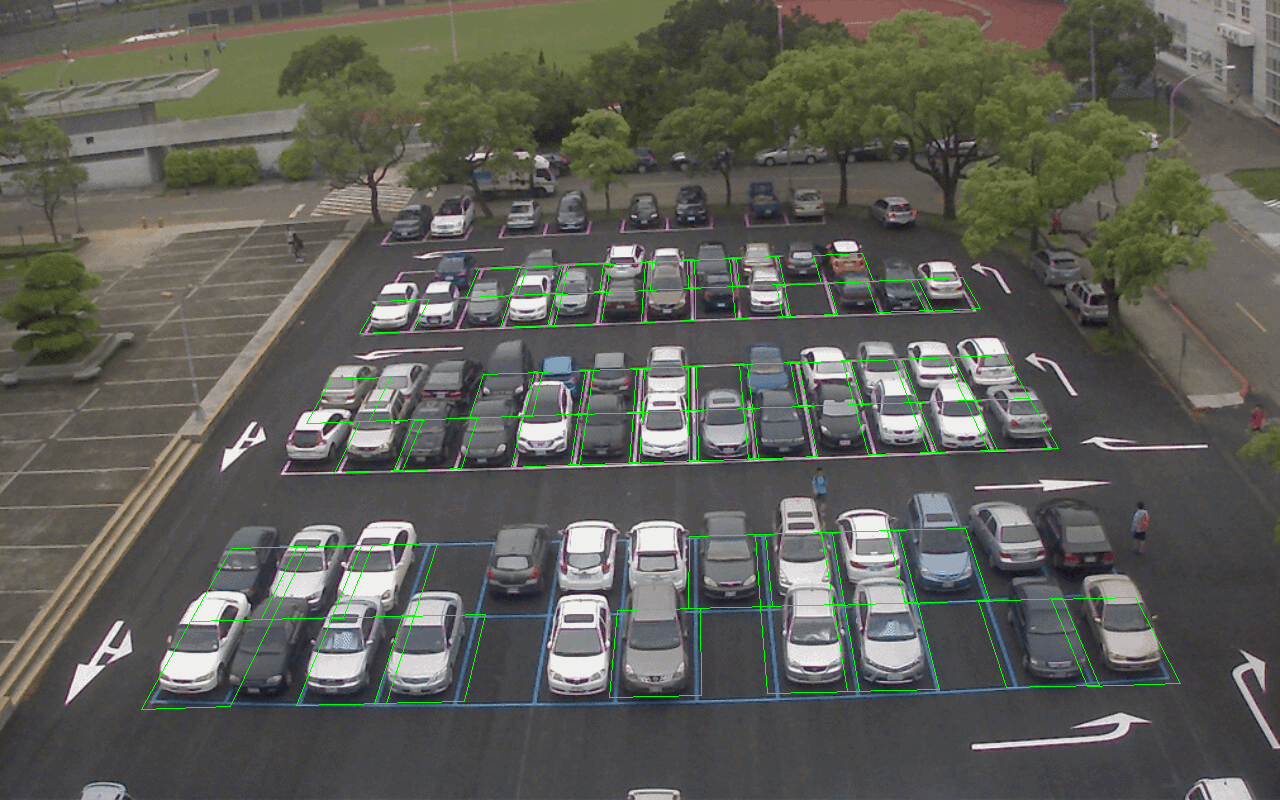
\includegraphics[width=0.75\textwidth]{figure/Adaboost_first_frame_6.png}
    \caption{The detection result of Adaboost with 6 classfiers}
\end{figure}

\begin{figure}[H]
    \centering
    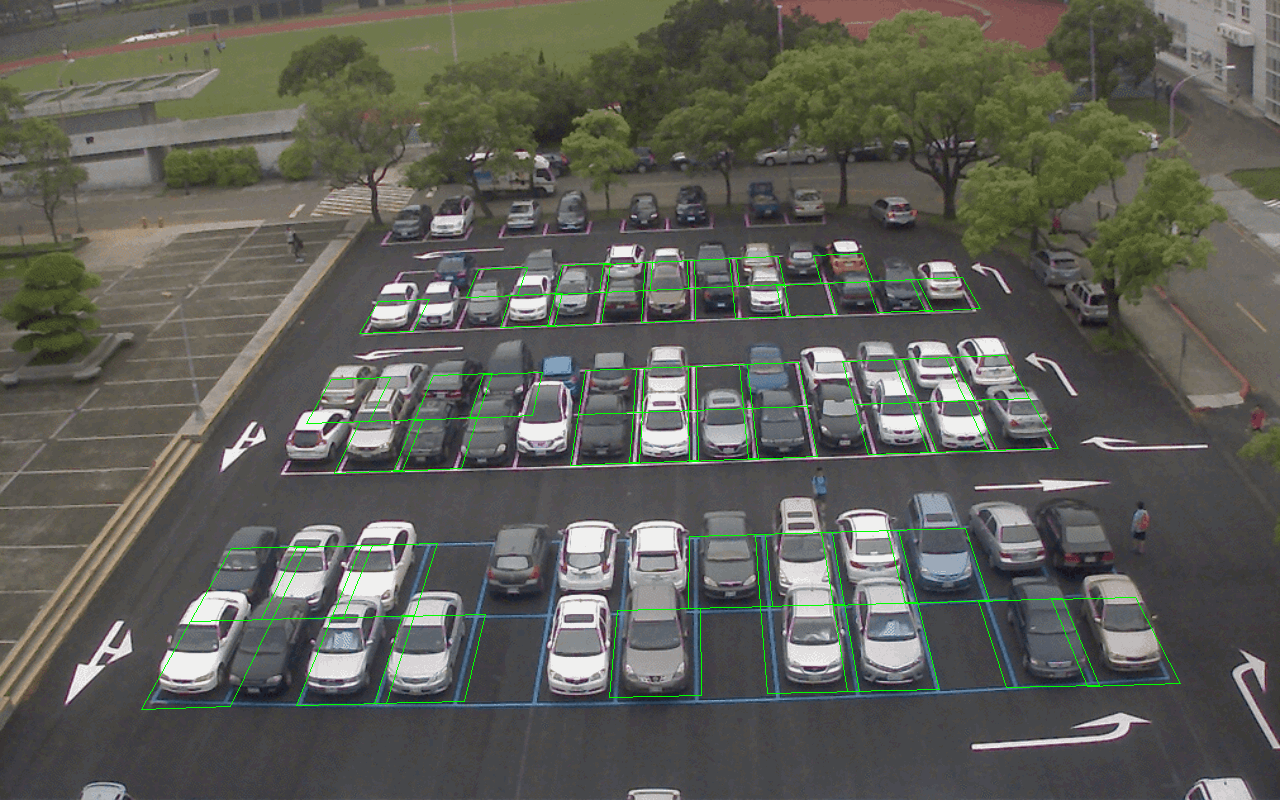
\includegraphics[width=0.75\textwidth]{figure/Adaboost_first_frame_8.png}
    \caption{The detection result of Adaboost with 8 classfiers}
\end{figure}

\begin{figure}[H]
    \centering
    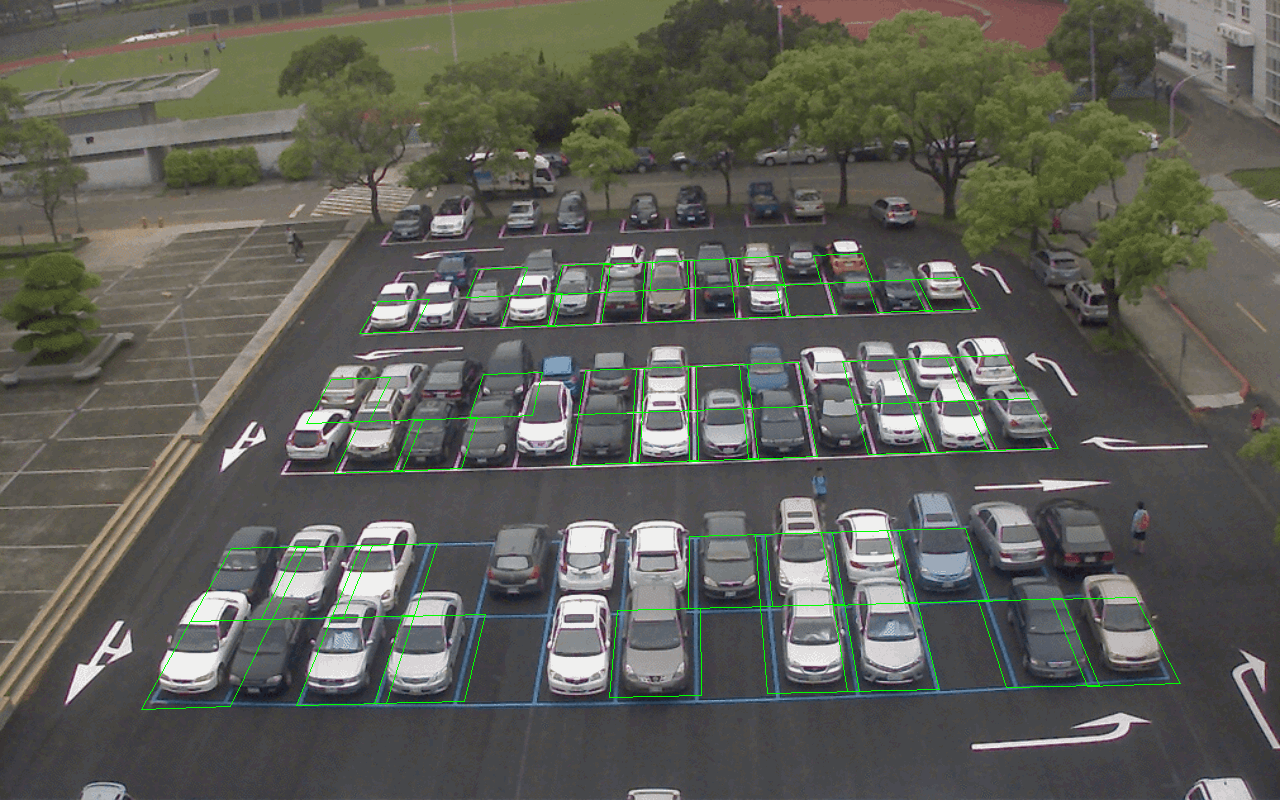
\includegraphics[width=0.75\textwidth]{figure/Adaboost_first_frame_10.png}
    \caption{The detection result of Adaboost with 10 classfiers}
\end{figure}

\begin{figure}[H]
    \centering
    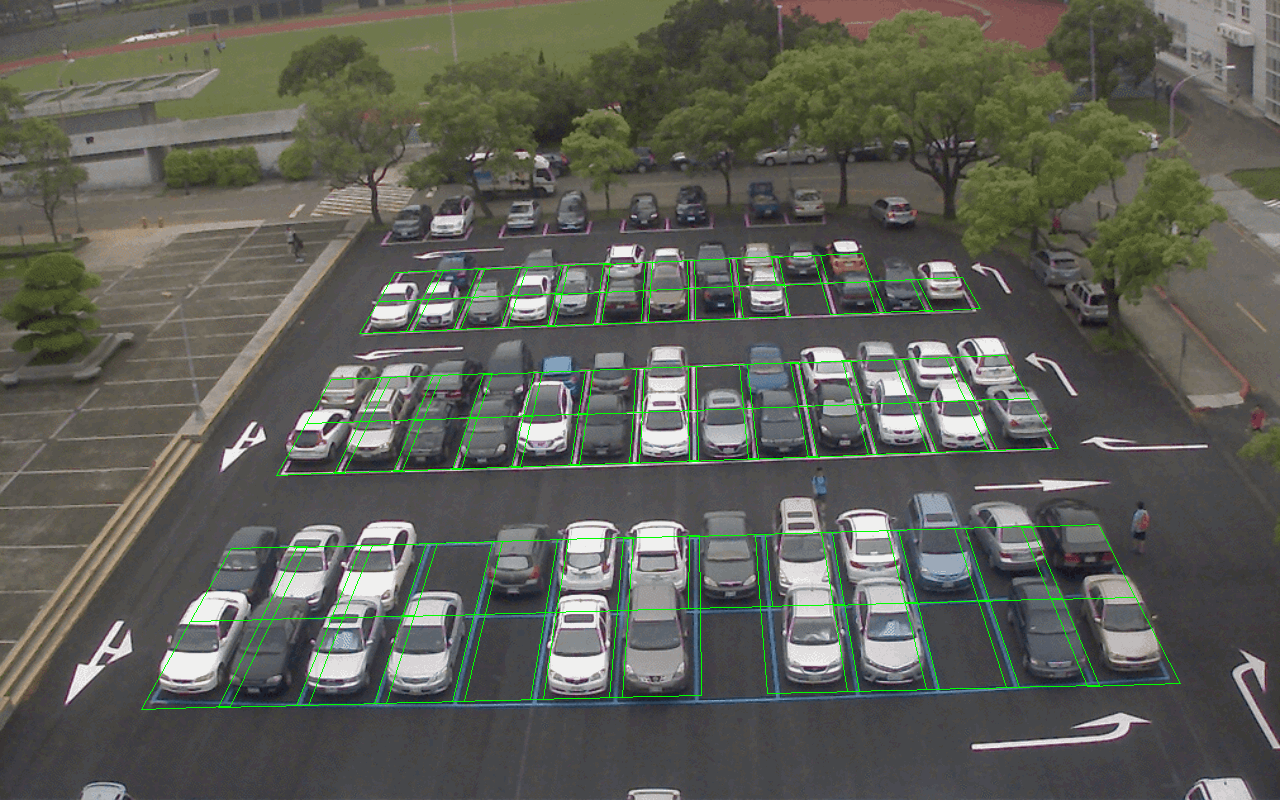
\includegraphics[width=0.75\textwidth]{figure/Yolov5_first_frame_1.png}
    \caption{The detection result of YOLOv5 with threshold set to 0.1}
\end{figure}

\begin{figure}[H]
    \centering
    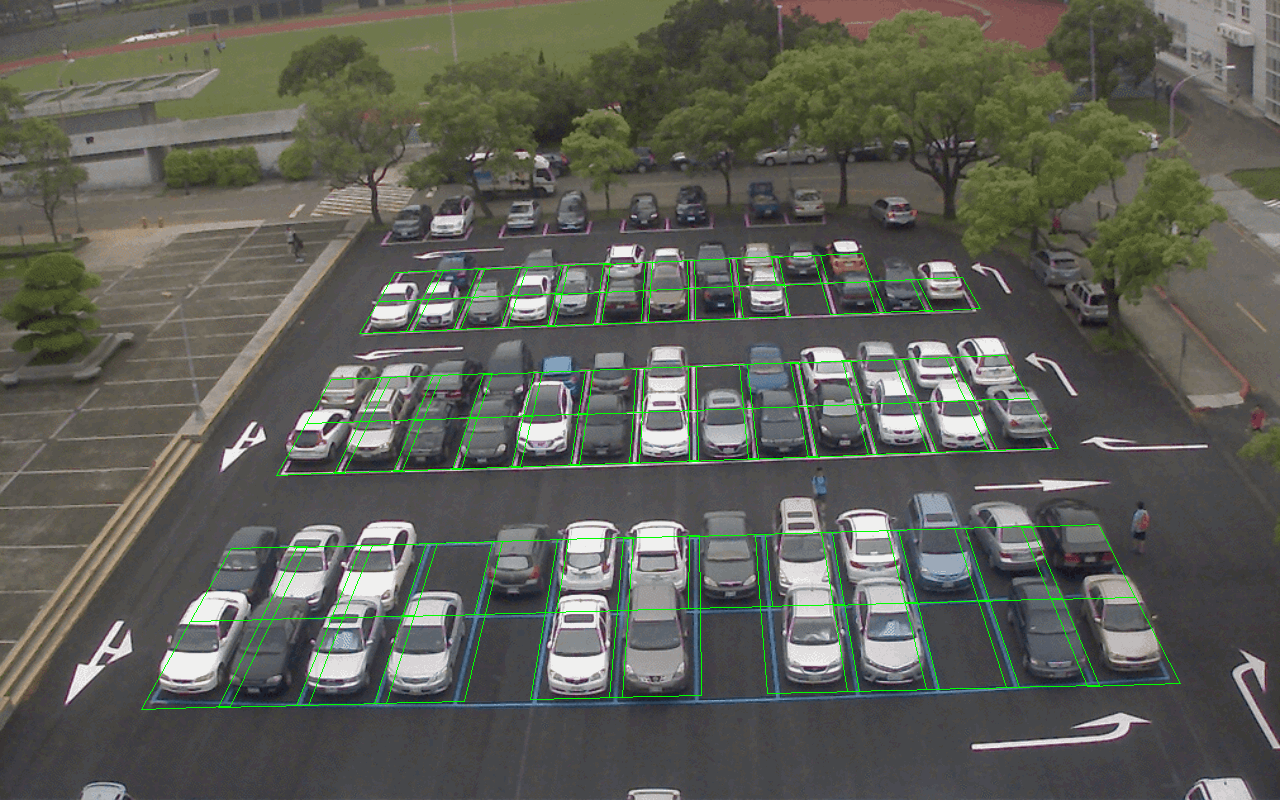
\includegraphics[width=0.75\textwidth]{figure/Yolov5_first_frame_2.png}
    \caption{The detection result of YOLOv5 with threshold set to 0.2}
\end{figure}

\begin{figure}[H]
    \centering
    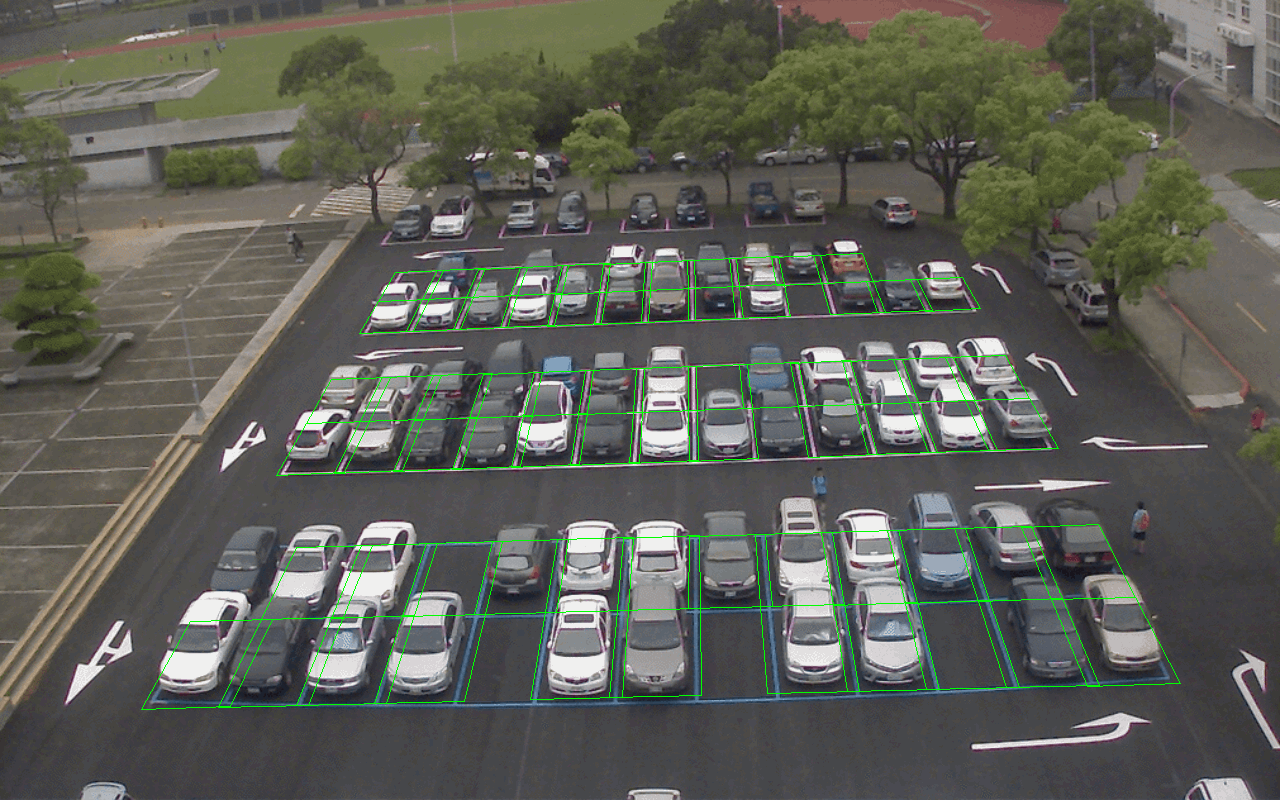
\includegraphics[width=0.75\textwidth]{figure/Yolov5_first_frame_3.png}
    \caption{The detection result of YOLOv5 with threshold set to 0.3}
\end{figure}


\begin{figure}[H]
    \centering
    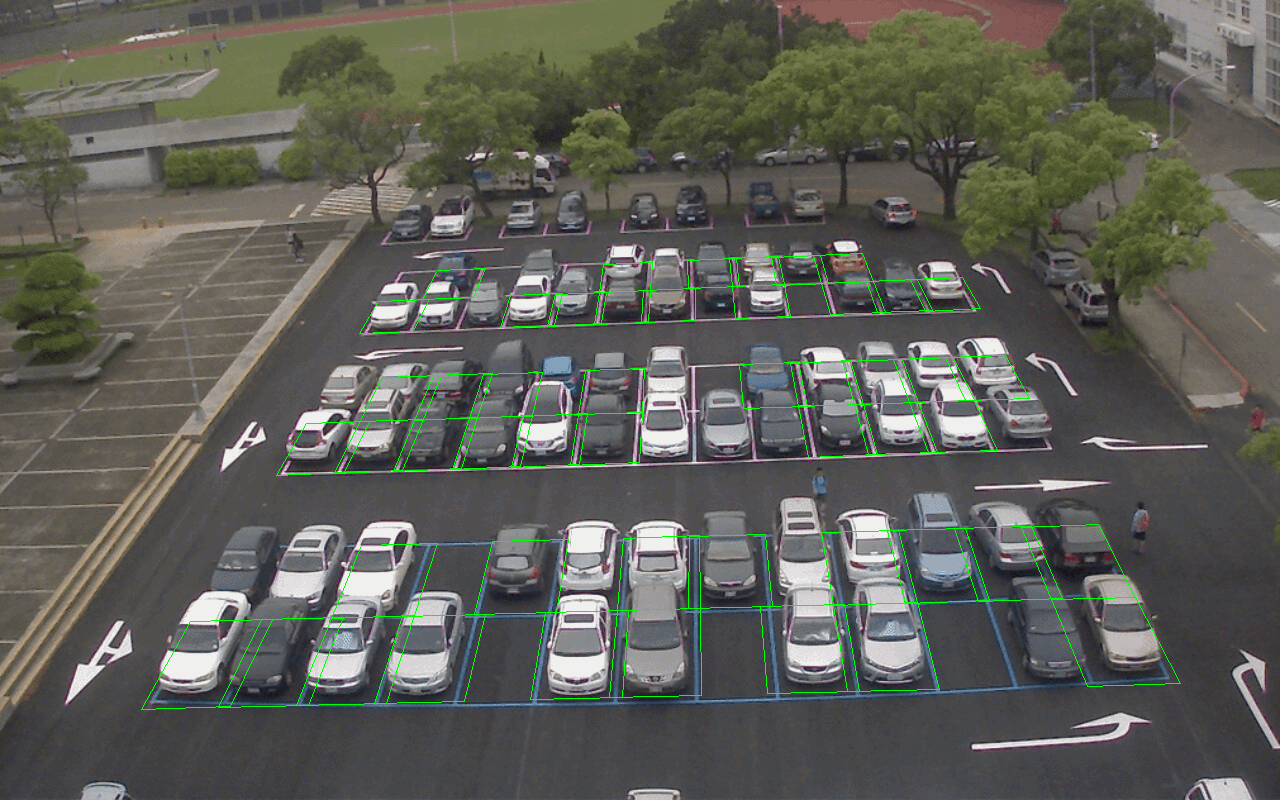
\includegraphics[width=0.75\textwidth]{figure/Yolov5_first_frame_4.png}
    \caption{The detection result of YOLOv5 with threshold set to 0.4}
\end{figure}


\begin{figure}[H]
    \centering
    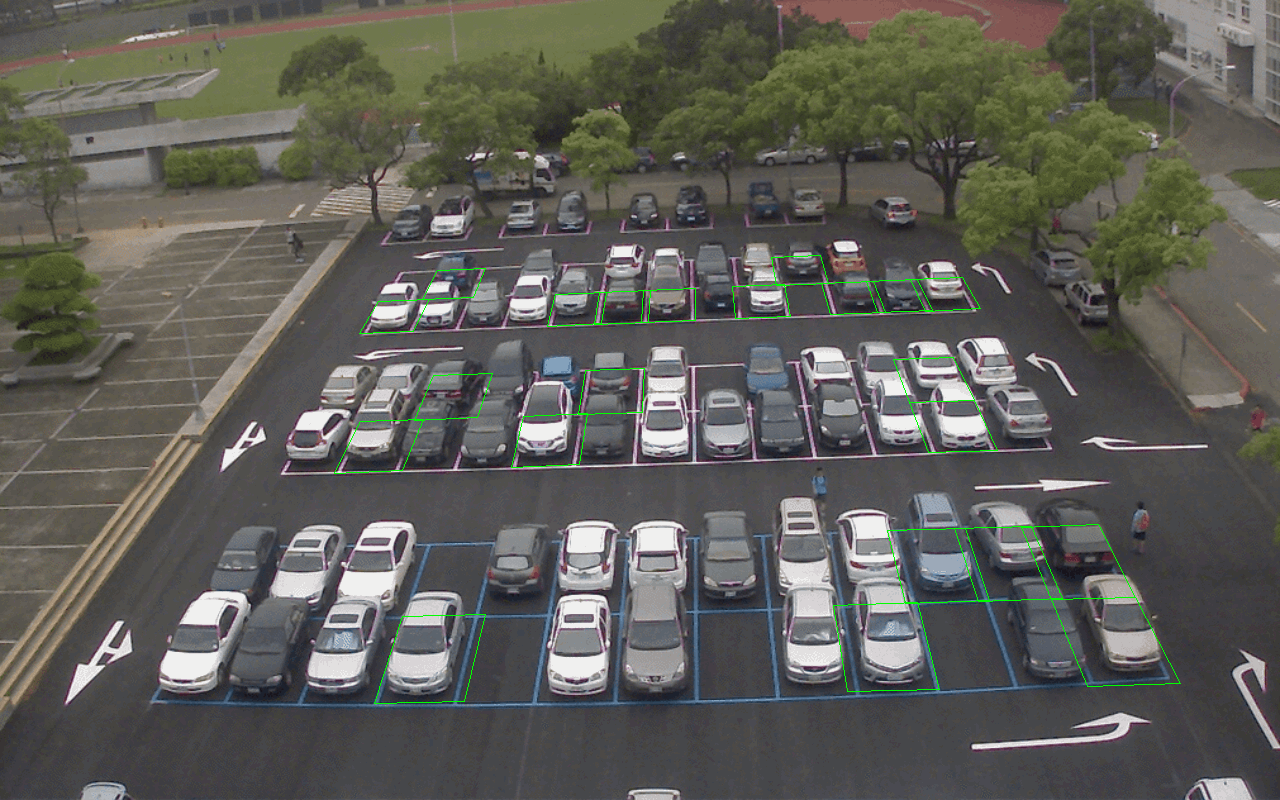
\includegraphics[width=0.75\textwidth]{figure/Yolov5_first_frame_5.png}
    \caption{The detection result of YOLOv5 with threshold set to 0.5}
\end{figure}

\begin{figure}[H]
    \centering
    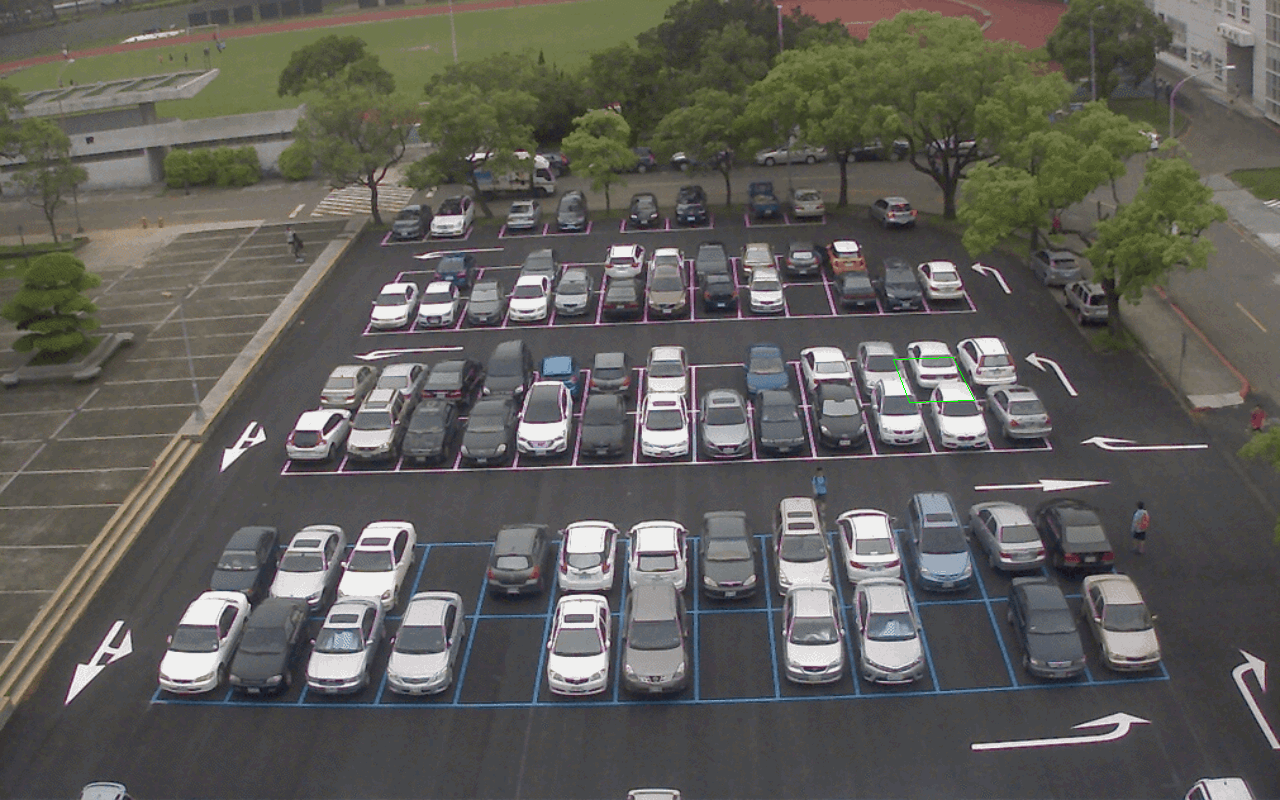
\includegraphics[width=0.75\textwidth]{figure/Yolov5_first_frame_6.png}
    \caption{The detection result of YOLOv5 with threshold set to 0.6}
\end{figure}

\subsubsection{Discussion}

As we can see in the plots and figures, the best model in this task is
the YOLOv5 whose confidence thresholds are set to 0.3.

This result is inconsistent with the results present in 
Section \ref{subsec:ada_comp} and Section \ref{subsec:yolo_comp}. 

I guess that this situation happened because in the real parking lot, 
most of the parking slots are occupied. 
Therefore, if we set the confidence threshold to a lower value(like 0.3), then the model 
will more likely to detect an occupied parking slot. This will make the model's performance better.
However, if the parking lot we are going to detect has less occupied parking slots,
setting a lower confidence threshold might not be a good idea. This may cause the detection results 
has lots of false positive samples.

In conclusion, I think the selection of the confidence threshold is actually hard. I suggest set
the confidence threshold to 0.5. Because if the parking lot is half-occupied (like in training 
and testing datasets), setting the confidence threshold to 0.5 will have the best performance.


\section{Problems}
\subsection{alpha = math.log(1.0/beta) ValueError: math domain error}
The original code in \texttt{adaboost.py} line 59 is 
\texttt{weights = weights / np.linalg.norm(weights)},
but the default normalization method used in np.linalg.norm is L2-Norm, 
which may lead some divide by zero problem in the calculation of alpha.
Therefore, I changed this line to \texttt{weights = weights / np.linalg.norm(weights, ord=1)}, 
which used the L1-Norm. After this change, the error in the title never shows up again.

\section{Bonus: Use HSV channel to detect occupied parkint slots}

\subsection{Plot the histogram of HSV channel of ``car'' and ``non-car'' datasets}

Out of curious, I plot the histogram of car and non-car training datasets HSV channels after converting
the image from RGB to HSV. 

The result is shown as Figure \ref{fig:hsv_h}, \ref{fig:hsv_s} and \ref{fig:hsv_v}.

\begin{figure}[H]
    \centering
    \begin{subfigure}[b]{0.45\textwidth}
        \centering
        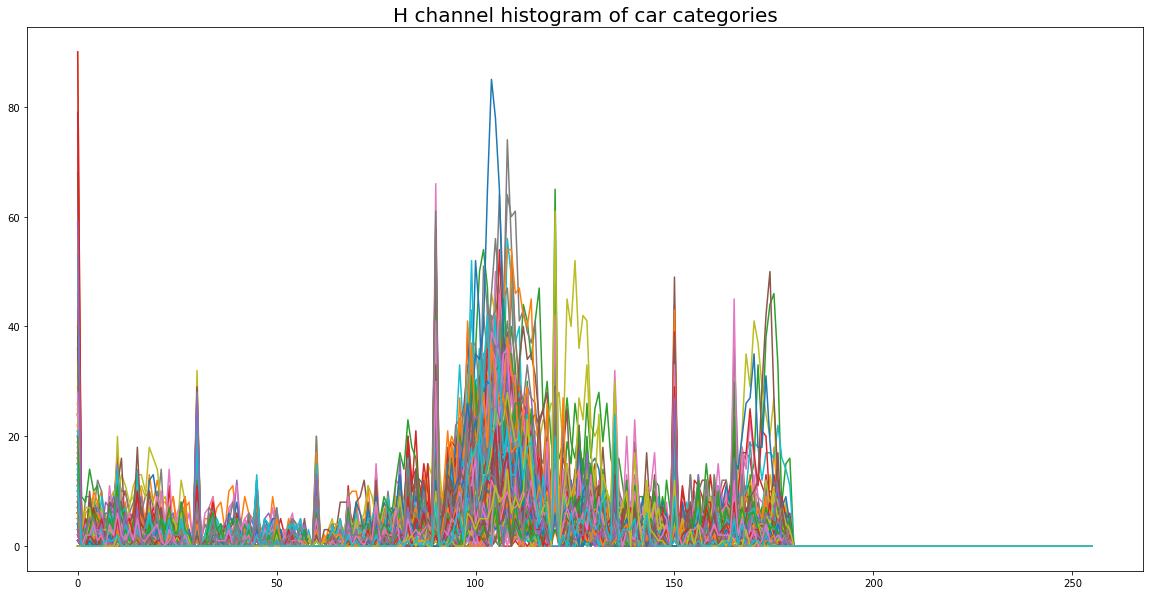
\includegraphics[width=\textwidth]{figure/H_car.png}
        \caption{Car}
    \end{subfigure}
    \hfill
    \begin{subfigure}[b]{0.45\textwidth}
        \centering
        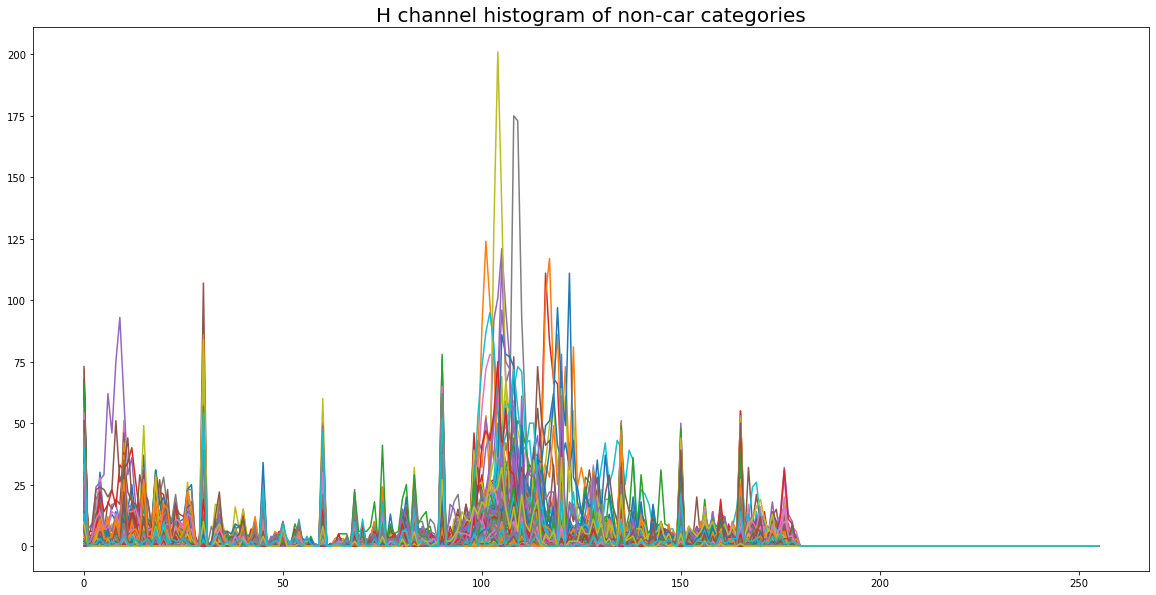
\includegraphics[width=\textwidth]{figure/H_noncar.png}
        \caption{Non-car}
    \end{subfigure}
    \caption{The H channel histogram of ``car'' and ``non-car'' images in training datasets.}
    \label{fig:hsv_h}
\end{figure}

\begin{figure}[H]
    \centering
    \begin{subfigure}[b]{0.45\textwidth}
        \centering
        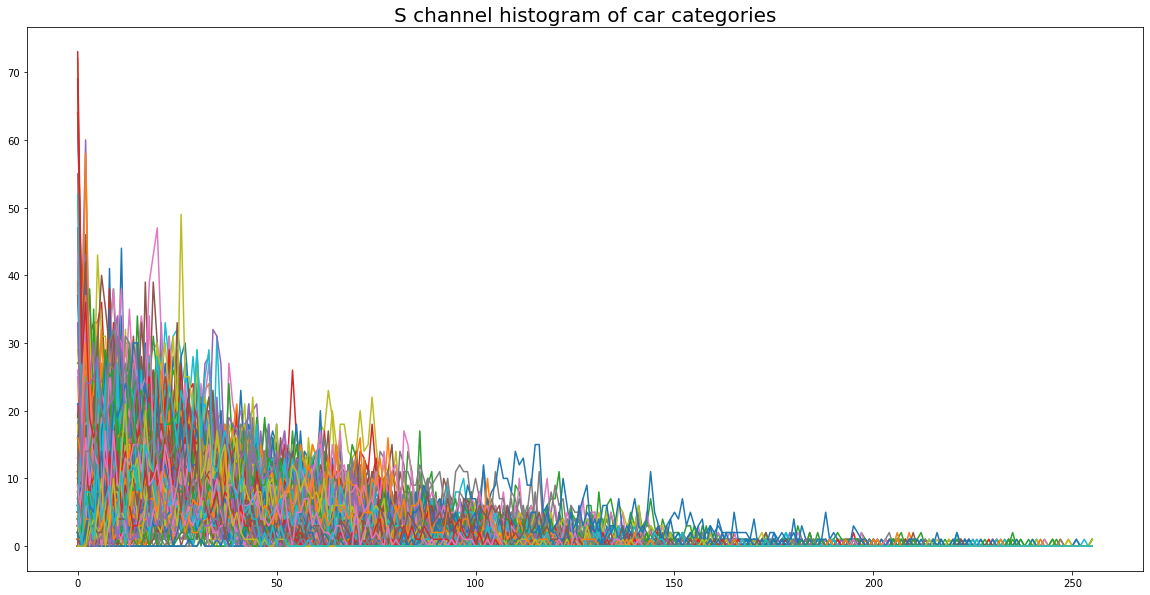
\includegraphics[width=\textwidth]{figure/S_car.png}
        \caption{Car}
    \end{subfigure}
    \hfill
    \begin{subfigure}[b]{0.45\textwidth}
        \centering
        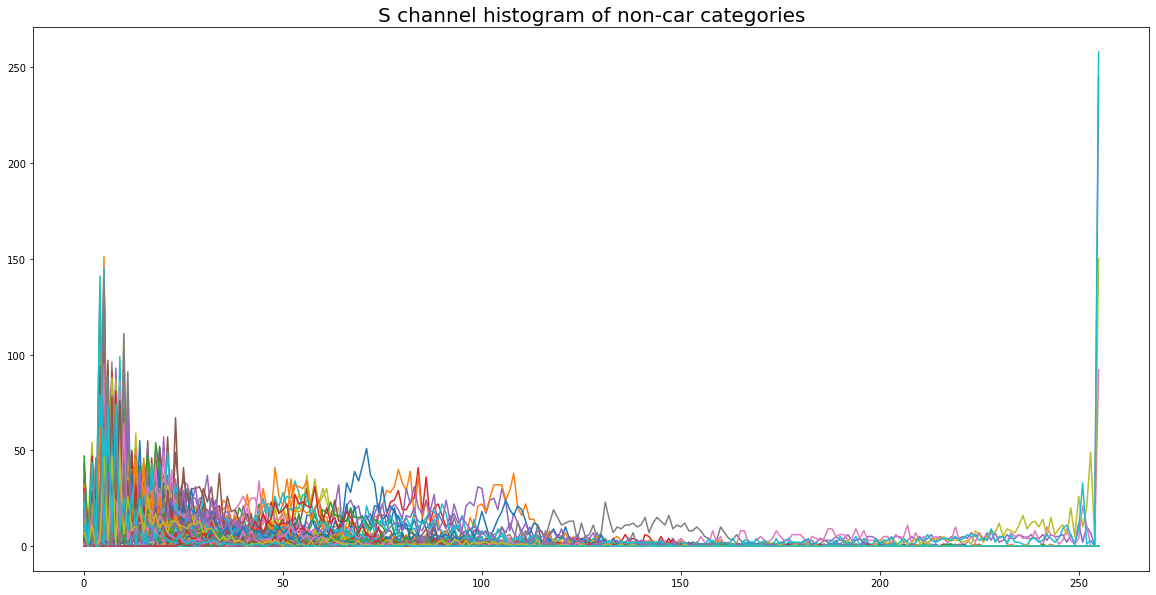
\includegraphics[width=\textwidth]{figure/S_noncar.png}
        \caption{Non-car}
    \end{subfigure}
    \caption{The S channel histogram of ``car'' and ``non-car'' images in training datasets.}
    \label{fig:hsv_s}
\end{figure}

\begin{figure}[H]
    \centering
    \begin{subfigure}[b]{0.45\textwidth}
        \centering
        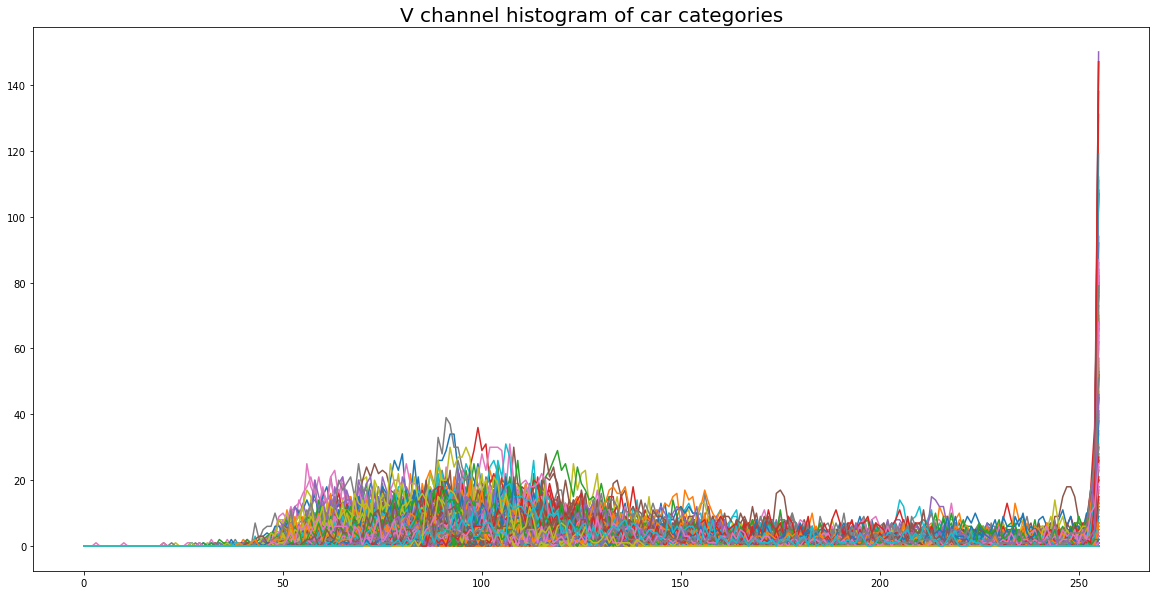
\includegraphics[width=\textwidth]{figure/V_car.png}
        \caption{Car}
    \end{subfigure}
    \hfill
    \begin{subfigure}[b]{0.45\textwidth}
        \centering
        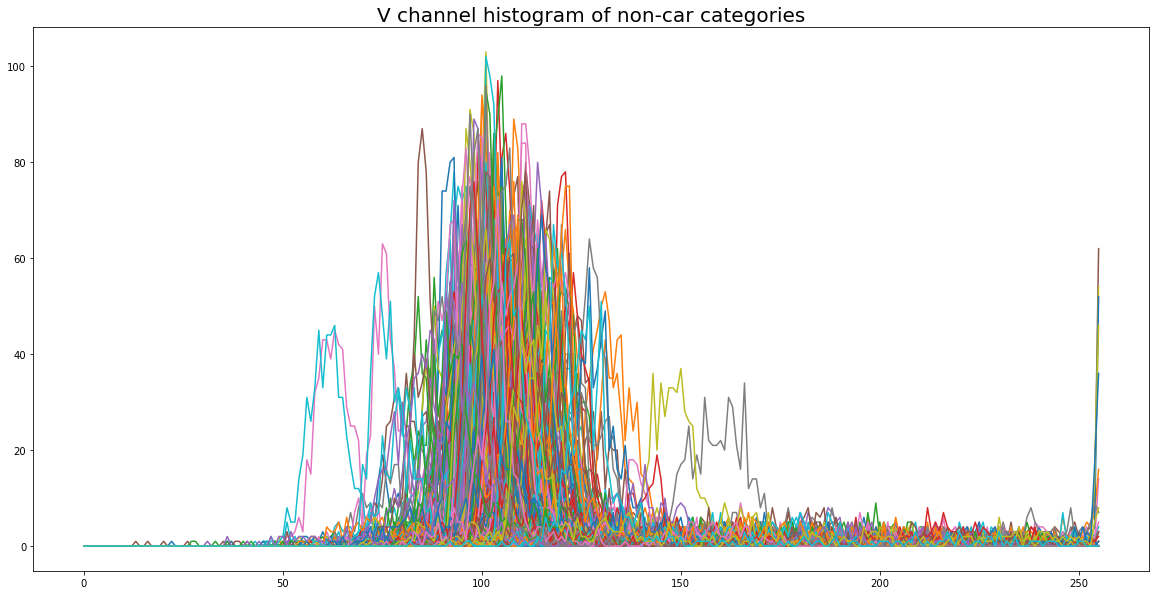
\includegraphics[width=\textwidth]{figure/V_noncar.png}
        \caption{Non-car}
    \end{subfigure}
    \caption{The V channel histogram of ``car'' and ``non-car'' images in training datasets.}
    \label{fig:hsv_v}
\end{figure}

As we can see, the V channel of ``car'' and ``non-car'' images have significant differences. 

Most of the ``non-car'' images have a peak intensity is in the range of $[40, 200]$ and their maximum y-value 
(number of pixels) are greater than $40$.

On the other hand, most of the ``car'' images' maximum y-values are less than $35$.

Therefore, we can use this feature to classify whether this parking slot is occupied or not. 
Next section will discuss how to write the actual code to make this method work.


\subsection{The detection code of the ``V-channel histogram'' method}

After conducting some experiments, I set the highest peak range to $[40, 200]$ and the threshold to 27. 
Below is the code I implemented to detect the parking slot using the ``V-channel histogram'' method.

\begin{code}
\captionof{listing}{classify function(\texttt{bonus/classify.py})}
\begin{minted}
import cv2
import numpy as np

def classify(img):
    v = img[:,:,2] # Extract the V channel from an HSV images
    hist_v = cv2.calcHist([v], [0], None, [256], [0, 256]) # Use cv2.calcHist to calculate the histogram.
    # If hist_v's highest peak occured in [40, 200] and its y-value is greater than 27, then we consider this parking slot isn't occupied
    if 40 <= np.argmax(hist_v) and np.argmax(hist_v) <= 200 and 27 <= np.max(hist_v):
        return False
    else:
        return True
\end{minted}
\end{code}

Because we need to convert images to HSV, I also edit \texttt{datasets.py} to convert images in advance.

\begin{code}
\captionof{listing}{\texttt{bonus/dataset.py}}
\begin{minted}
import os
import cv2

def loadImages(dataPath):
    """
    Load all Images in the folder and transfer a list of tuples. 
    The first element is the numpy array of shape (m, n) representing the image.
    (remember to resize and convert the parking space images to 36 x 16 grayscale images.) 
    The second element is its classification (1 or 0)
        Parameters:
        dataPath: The folder path.
        Returns:
        dataset: The list of tuples.
    """
    # Begin your code (Part 1)
    dataset = [] # Declare an empty list to save the grayscale images

    # Process images in "car" directory
    for item in os.listdir(os.path.join(dataPath, "car")): # Use os.path.join to generate paths
        img = cv2.imread(os.path.join(dataPath, "car", item)) # Read image from files
        img = cv2.resize(img, (36, 16)) # Resize the image from (360, 160) to (36, 16)
        img = cv2.cvtColor(img, cv2.COLOR_BGR2HSV) # Convert image to HSV image
        data = (img, 1) # Create a tuple to store image and label and 
        # because all images in "car" folder is the occupied parking space, the label is set to 1
        dataset.append(data) # Append the tuple to the dataset list
    
    for item in os.listdir(os.path.join(dataPath, "non-car")): # Do the same thing as above but this time is for "non-car" folder
        img = cv2.imread(os.path.join(dataPath, "non-car", item))
        img = cv2.resize(img, (36, 16))
        img = cv2.cvtColor(img, cv2.COLOR_BGR2HSV)
        data = (img, 0) # Not occupied parking space, label is set to 0
        dataset.append(data)
    # End your code (Part 1)
    
    return dataset    
\end{minted}
\end{code}

\subsection{Results}

\subsubsection{Comparison on testing datasets}

\begin{table}[H]
    \centering
    \caption{Performance of Adaboost, YOLOv5 and V-Channel Method on testing datasets}
    \begin{tabular}{@{}ccccccc@{}}
    \toprule
    Model    & FP Rate (\%)  & FN Rate (\%)  & Accuracy (\%)  & Precision (\%) & Recall (\%)    & F1-score       \\ \midrule
    Adaboost & 8.33          & 19.33         & 86.17          & 91.67          & 82.58          & 86.89          \\
    YOLOv5   & \textbf{1.67} & \textbf{1.00} & \textbf{98.67} & \textbf{98.33} & \textbf{98.99} & \textbf{98.66} \\ 
    V-Channel & 3.33 & 1.33 & 97.6 & 96.67 & 98.64 & 97.64 \\ \bottomrule
    \end{tabular}
    \label{tab:com_v}
\end{table}

As we can see in Table \ref{tab:com_v}, though our method's performance is slightly worse than YOLOv5
, the advantage of V-channel method is that the detection speed is much faster than YOLOv5, 
and running the algorithm does not require an expensive GPU or chip. 

\subsubsection{Comparison on an real parking lot}

\begin{figure}[H]
    \centering
    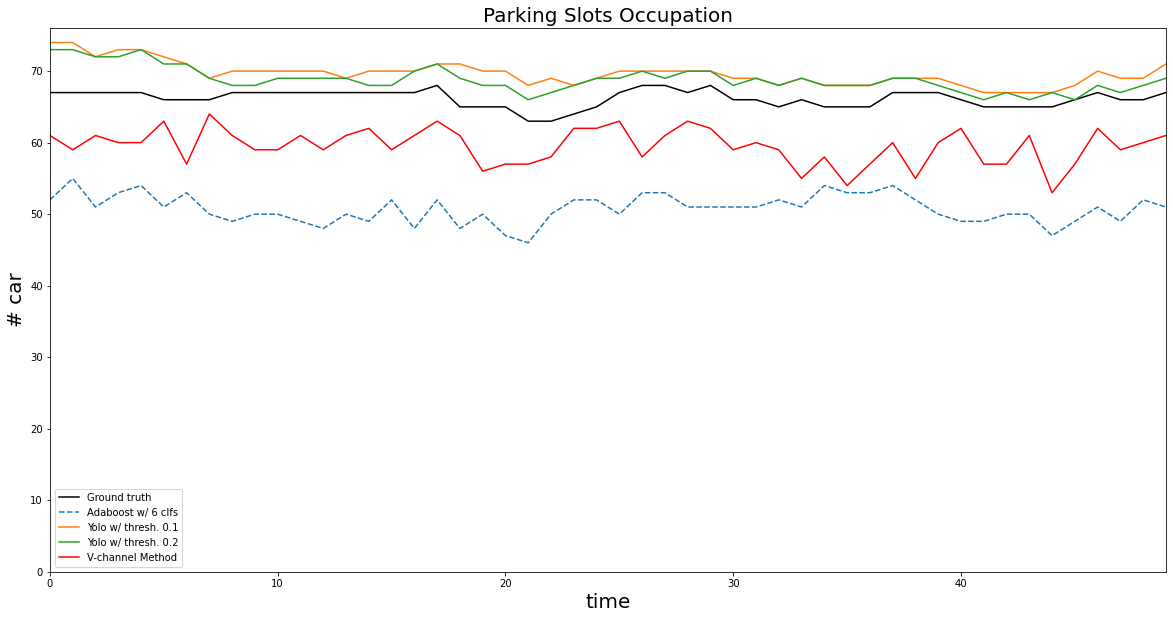
\includegraphics[width=0.75\textwidth]{figure/Parking_Slots_Occupation_v.png}
    \caption{The number of occupied parking slots detected by Adaboost(with 6$\sim$10 classifers)
    , YOLOv5(with threshold 0.1$\sim$0.4), V-channel method and the ground truth}
\end{figure}

\begin{figure}[H]
    \centering
    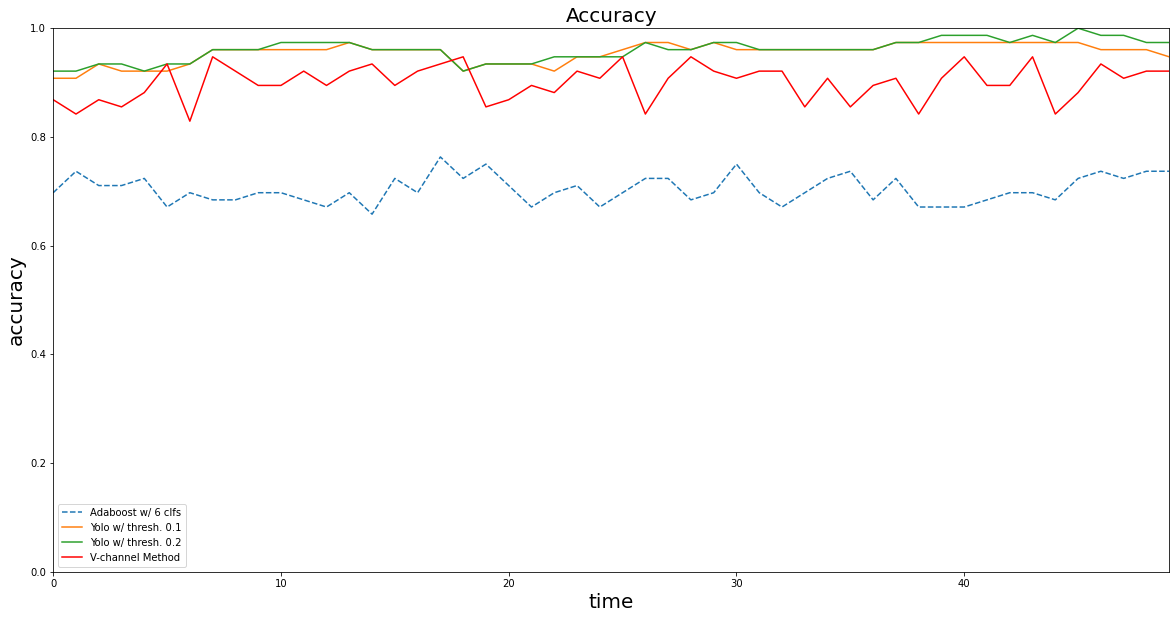
\includegraphics[width=0.75\textwidth]{figure/Accuracy_v.png}
    \caption{The Accuracy of Adaboost(with 6$\sim$10 classifers)
    , YOLOv5(with threshold 0.1$\sim$0.4) and V-channel method}
\end{figure}

\begin{figure}[H]
    \centering
    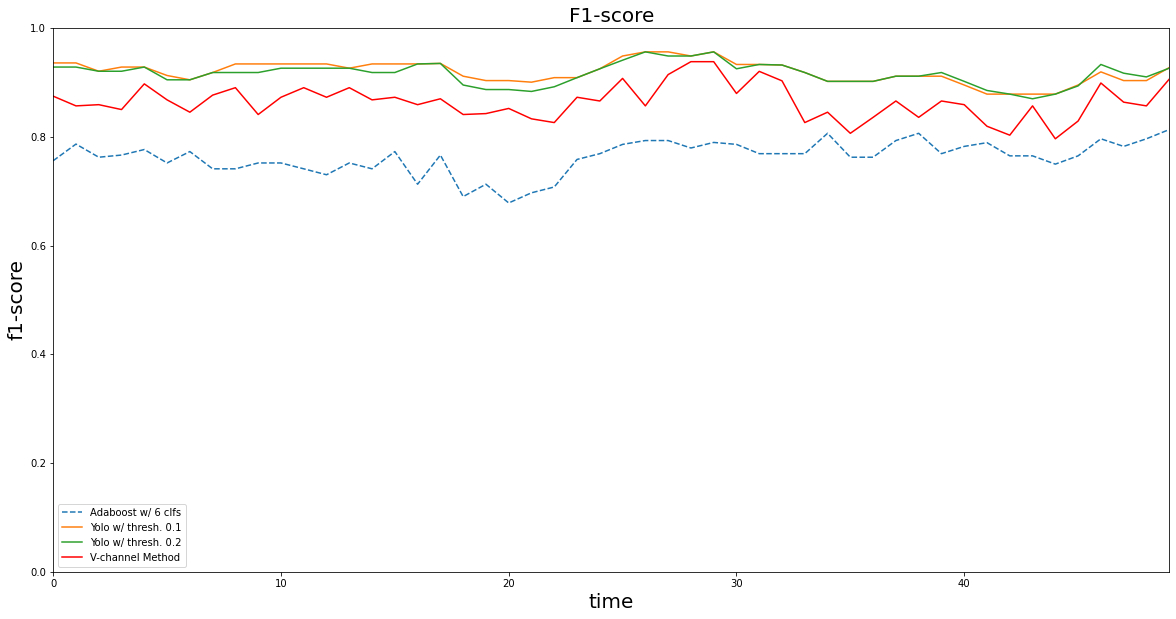
\includegraphics[width=0.75\textwidth]{figure/F1-score_v.png}
    \caption{The F1-score of Adaboost(with 6$\sim$10 classifers)
    , YOLOv5(with threshold 0.1$\sim$0.4) and V-channel method}
\end{figure}

\begin{figure}[H]
    \centering
    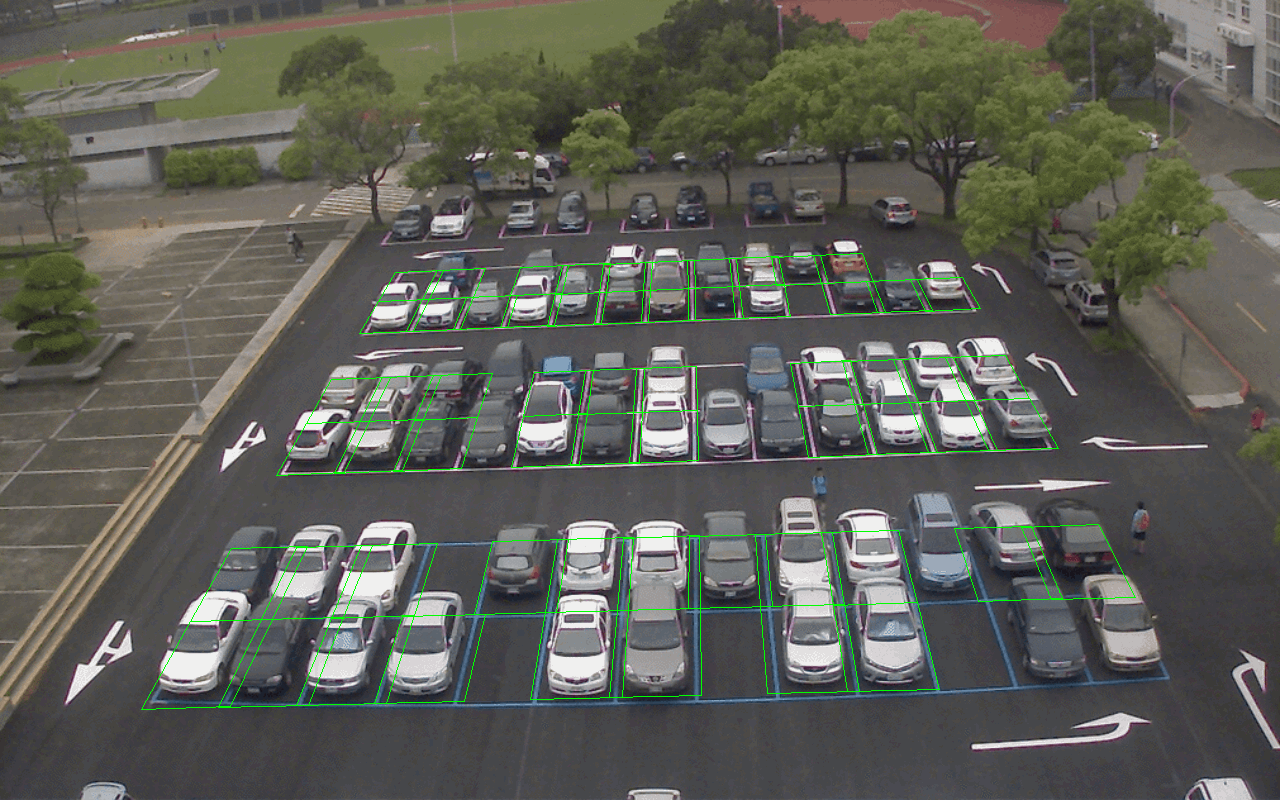
\includegraphics[width=0.75\textwidth]{figure/CV_first_frame.png}
    \caption{The detection result of V-channel method}
\end{figure}

\end{document}